\chapter{Problem analysis} \label{chapter:problem-analysis}
In the problem analysis chapter we explore the feature engineering methods and machine learning algorithms for fault diagnostics. The basis we build upon is the domain knowledge of mechanical engineers in vibration signal measurement and its evaluation.

\section{Condition monitoring} \label{section:condition-monitoring}
All rotating machinery eventually fails because of the long-term strain on the individual parts, inadequate workmanship, installation, or operational procedures. In the end, these factors cause the equipment not to fulfill its intended functionality. Many instrumentation methods are practiced to reveal evolving faults: vibration and acoustic noise monitoring, electric supply line measurements, thermography, oil and particle analysis, ultrasonic testing, etc. Vibration signals are the preferred tool for rotating machinery monitoring~\cite{mohanty_machinery_2015}.

The defect needs to be repaired or replaced, preferably without significant production downtime, further damage to the other attached elements, or any endangerment of the responsible personnel. The maintenance strategies are chosen according to the machine's importance as a result of potential failure's impact on the system. The guide to set appropriate maintenance procedures is outlined in the IEC~60706-2 standard and involves reliability-centered maintenance analysis~\cite{el-thalji_predictive_2019}.

\subsection{Maintenance strategies}
There are three different approaches to maintenance across the industry: \textbf{reactive, preventive, and predictive}~\cite{scheffer_practical_2004}. In general, the more sophisticated methods are beneficial in a high-stakes environment. The unexpected machine shutdown can have a negative economic impact on the enterprise which results in decreased product quality and demands for spare parts to be ready in the supply inventory at all times. In certain situations, it suffices to utilize a simpler maintenance program, but predictive maintenance gains attraction in Industry 4.0 to optimize usage of assets~\cite{cinar_machine_2020}.

\textbf{Reactive maintenance} allows machinery to run until a complete failure which is the most inappropriate way to maintain the production line, but it is straightforward enough. It requires a large stock of replacement parts on-site. Any breakage inflicts crisis management upon the plant \cite{scheffer_practical_2004}. On-demand repairs are justified when short downtime is acceptable, full and swift replacement of a broken machine with a backup is possible, or there is a negligible threat to the surrounding environment from failure~\cite{ziaran_technicka_2013}.

\textbf{Preventive maintenance} is performed before any issue is detected. Maintenance occurs at regular intervals derived from a predetermined period in the calendar or expected machine running time and its mean time to failure (MTTF). The schedule is crucial but can result in components being replaced in good condition, creating waste. The parts can occasionally stay in operation too long, and the machine breaks as a result. Conservative planning is usually the norm to keep the machines in perfect shape. Therefore, more frequent interventions are required~\cite{mohanty_machinery_2015}.

\textbf{Predictive maintenance} (PdM) known also as condition-based maintenance (CbM), improves the predictability of reactive maintenance and eliminates waste in overall resource utilization of cautious prevention. The machine downtime is scheduled after the detection of unhealthy trends in fault monitoring with sensors and the identification of troublesome components.

A measurable decrease in effectiveness allows us to order necessary parts in advance and organize repairs of several machines at a convenient time. The missed detection leads to increased costs compared to previous methods and raises the expectation that faults are distinguishable among themselves~\cite{davies_handbook_2012}.

\begin{figure}[ht]
	\centering
	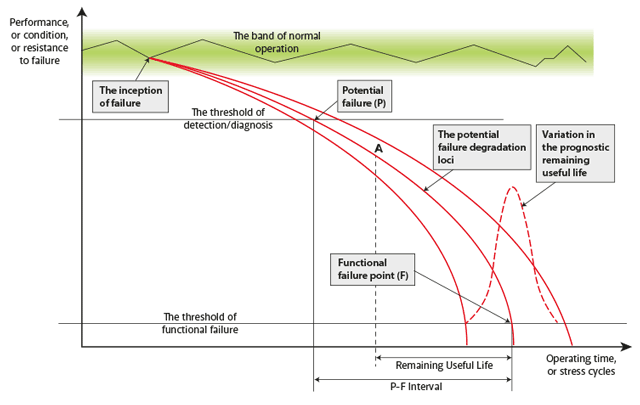
\includegraphics[width=\textwidth]{assets/analysis/P-F-Curve.png}
	\caption{P-F curve represents the evolution of the asset's health~\cite{jennions_integrated_2011}}
	\label{fig:p-f-curve}
\end{figure}

The \emph{P-F curve} is a widespread representation of equipment's degradation over time based on historical records (Fig.~\ref{fig:p-f-curve}). Corrective action should be taken between the event of potential failure (P), when the fault detection is activated, and functional failure point (F) in the P-F interval~\cite{bousdekis_enterprise_2021}. These division points are not set precisely but have a statistical distribution.

The \emph{Remaining Useful Life} (RUL) of the specific running machine in the given instance can be merely estimated analytically, with the survival probabilities of the individual components, based on the model of the ``run-to-failure'' history and usage parameters~\cite{okoh_overview_2014}. Predictive condition monitoring aims to extend the lifespan to the maximum by predicting expected RUL.

\begin{figure}[ht]
	\centering
	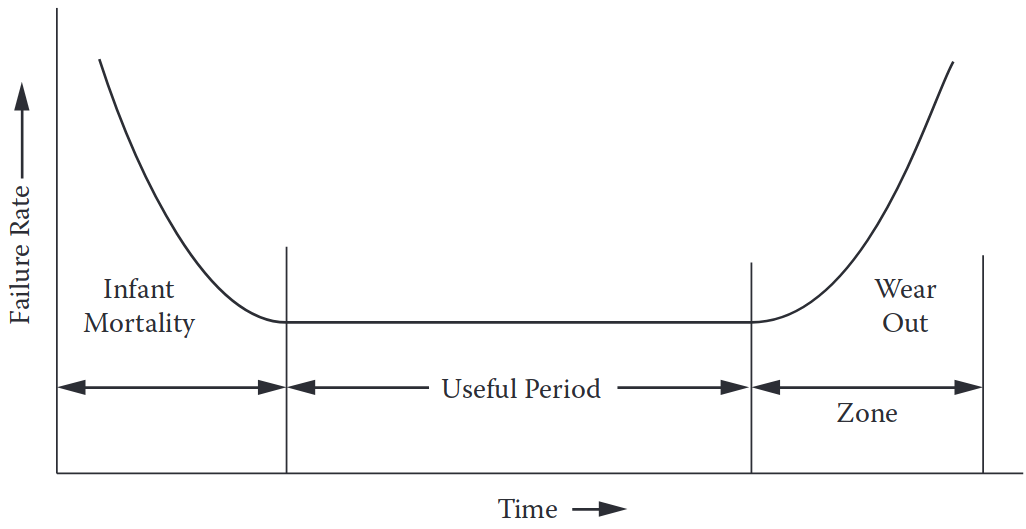
\includegraphics[width=0.6\textwidth]{assets/analysis/bath-tub-curve.png}
	\caption{Bathtub curve~\cite{mohanty_machinery_2015}}
	\label{fig:bathtub-curve}
\end{figure}

A high failure rate is present at the worn-out stage when the parts are fatigued or corroded. It can also be registered in the early stages soon after assembly. Manufacturing or material defects, inadequate installation, or improper start-up procedures are all suspected causes. During the stable middle phase, malfunction can occur after the machine's excessive overload. The time plot to failure rate is known as the bathtub curve~(Fig.~\ref{fig:bathtub-curve}).

\subsection{Vibration fault types}
Mechanical problems during machinery operation bring about vibrations in many instances. Therefore, vibroacoustic diagnostics is considered as one of the most important methods in early component fault identification~\cite{ziaran_technicka_2013}.

The cause of vibration comes out of the changing force in its magnitude or direction. The most emerging defects can be encompassed by explaining the deficiencies of the mechanical structure. These defects are broadly categorized as \textbf{unbalance, misalignment, looseness, eccentricity, deformation, crack, and influence of the external force} (friction)~\cite{davies_handbook_2012}. It is important to stress that our concern are not the underlying deformities in mechanical parts but the correct fault classification based on the signal waveform.

\begin{figure}[ht]
	\centering
	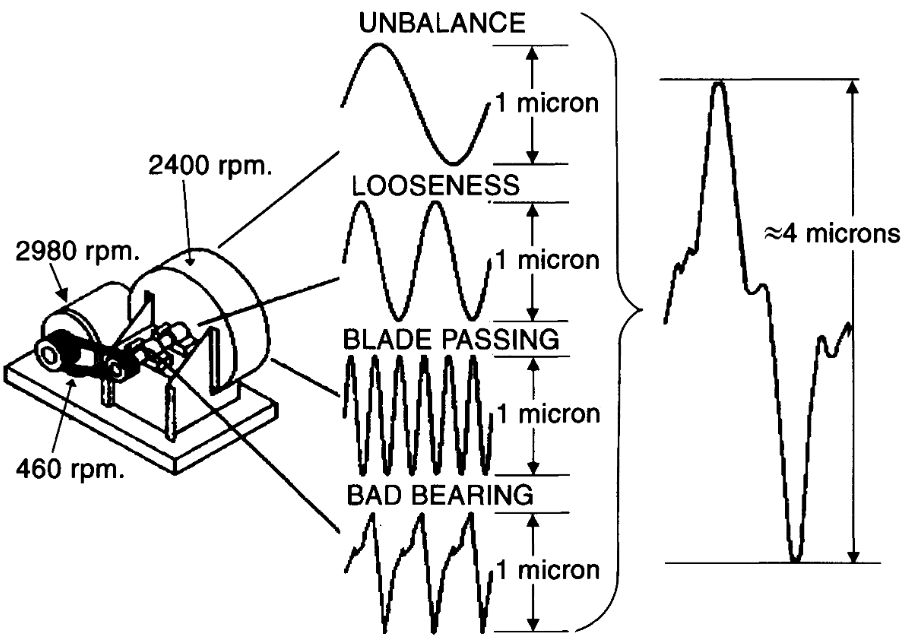
\includegraphics[width=0.6\textwidth]{assets/analysis/complex-vibrations.png}
	\caption{Complex machinery vibrations~\cite{davies_handbook_2012}}
	\label{fig:machinery-vibrations}
\end{figure}

Rotating machine disorders exhibit frequency signatures at various ranges in the frequency spectrum with supplementary symptoms carried in phase signal. Most of the occurring faults can be tied to the main rotational speed of the component under investigation (Fig.~\ref{fig:machinery-vibrations})~\cite{davies_handbook_2012}. Imbalance, misalignment, and looseness normally appear at frequencies up to 300 Hz. These low-frequency faults are associated with the movement of the shaft and primarily coincide with revolution speed and its harmonics. Bearing and gearbox defects in the late stages of development, show up in the range between 300 Hz and 1 kHz. Higher frequencies, measured traditionally to a limit of 10 kHz, help notice the faults in bearings even sooner~\cite{torres_automatic_2022}.

One of the methods vibration experts utilize in the identification of the damaged part, according to the frequency spectrum, is \textbf{order analysis}. The excessive peaks in harmonic frequencies are of interest. Harmonics are integer multiples of fundamental frequency (1x rpm)~(Tab.~\ref{tab:vibration-causes}):

\begin{table}[h]
\renewcommand{\arraystretch}{1.2}
\begin{adjustbox}{width=\columnwidth,center}
\begin{tabular}{|ll|l|l|}
\hline
\multicolumn{2}{|l|}{\textbf{Frequency content}}                            & \textbf{Likely reason}                                                                                                     & \textbf{Other causes}                                                                                                                          \\ \hline
\multicolumn{1}{|l|}{\multirow{4}{*}{Synchronous}} & 1 x rpm                & Imbalance                                                                                                                & \begin{tabular}[c]{@{}l@{}}Eccentric journals\\ Bent shaft / Misalignment\\    (high axial vibration)\\ Bad belt (if rpm of belt)\end{tabular} \\ \cline{2-4}
\multicolumn{1}{|l|}{}                             & 2 x rpm                & Looseness                                                                                                                & \begin{tabular}[c]{@{}l@{}}Misalignment \\    (high axial vibration)\\ Cracked rotor\\ Bad belt (if rpm of belt)\end{tabular}                  \\ \cline{2-4}
\multicolumn{1}{|l|}{}                             & 3 x rpm                & Misalignment                                                                                                             & and axial looseness                                                                                                                             \\ \cline{2-4}
\multicolumn{1}{|l|}{}                             & Many x rpm             & \begin{tabular}[c]{@{}l@{}}Bad gears\\ Severe looseness\end{tabular}                                                     & \begin{tabular}[c]{@{}l@{}}Gear teeth x rpm\\ Fan blade count x rpm\end{tabular}                                                               \\ \hline
\multicolumn{1}{|l|}{Sub-synchronous}                 & \textless 1 x rpm      & Oil whirl                                                                                                                & \begin{tabular}[c]{@{}l@{}}Bad drive belt\\ Background\\ Resonance\end{tabular}                                                                \\ \hline
\multicolumn{1}{|l|}{Non-synchronous}              & \multicolumn{1}{c|}{-} & \begin{tabular}[c]{@{}l@{}}Electrical problems (x 50 Hz)\\ Reciprocating forces\\ Aerodynamic forces \\ Bad antifriction bearings\end{tabular} & Rubbing \\ \hline
\end{tabular}
\end{adjustbox}
\caption{Expert observed likely vibration causes (based on~\cite{davies_handbook_2012,ziaran_technicka_2013,noauthor_iso_2002})}
\label{tab:vibration-causes}
\end{table}

Because of inherent tolerances in machine manufacturing and assembly, the rotational frequency always manifests itself, even in baseline signature~\cite{davies_handbook_2012, noauthor_iso_2002}. In the most likely scenario, some faults appear as compared to rotational frequency solely in \textbf{synchronous, subsynchronous, or non-synchronous components}. The defects can occur in a predictable combination of the ones mentioned. Other common patterns experts look for are modulation sidebands typical for bearings and gears extractable with cepstrum analysis~\cite{ziaran_technicka_2013}. Procedures relying on elimination narrow down unrelated causes effectively.

The mechanical properties of bearings are instrumental in identifying the characteristic frequencies of their components~\cite{mohanty_machinery_2015, ziaran_technicka_2013}. Bearings are composed of outer and inner circular races between which the rolling elements are held inside the cage to avoid mutual contact~(Fig.\ref{fig:bearing-parts}). The developing scratches or pits can appear as increases in amplitude around characteristic frequencies and their harmonics but sometimes this is not enough for accurate diagnostics~\cite{brito_fault_2021}.

\begin{figure}[h]
    \centering
    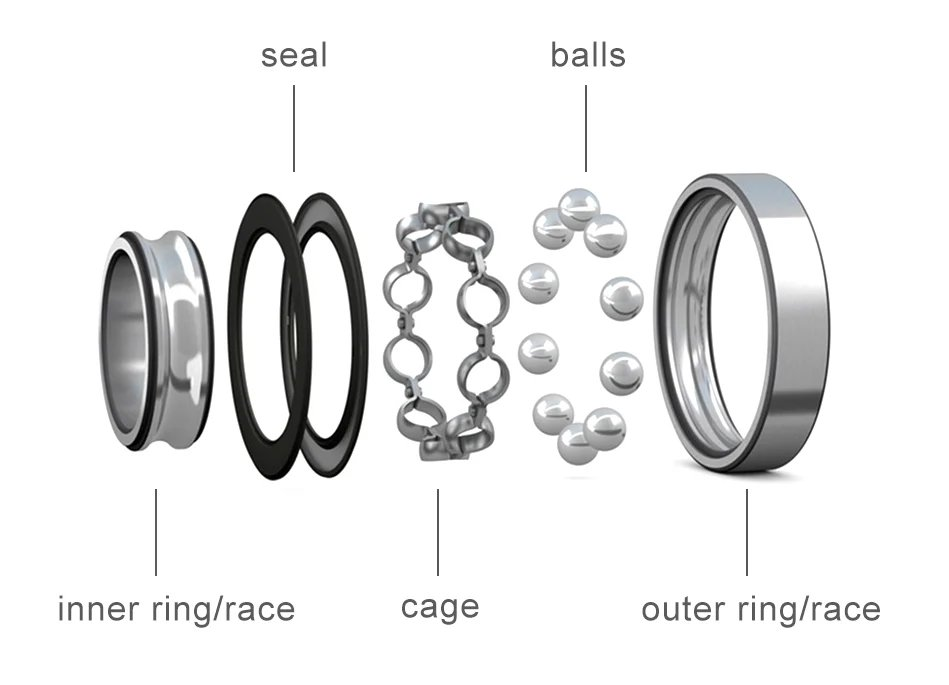
\includegraphics[width=0.7\textwidth]{assets/analysis/bearing-parts.jpg}
    \caption{Bearing parts~\cite{lu_what_is_ball_bearing_2023}}
    \label{fig:bearing-parts}
\end{figure}

The table \ref{tab:bearing-defect-features} provides formulas for rolling bearing defect frequencies at rotational speed $f_s$ where $n$ is a number of rolling elements, $d$ is the average of outer and inner ring diameters, and contact angle $\beta$. Because the frequencies of components depend on shaft rotational speed the values are supplied as its multiplication factors alongside datasets.

\begin{table}[h]
\centering
\renewcommand{\arraystretch}{2}
\begin{tabular}{|l|l|l|l|}
\hline
\textbf{Feature}            & \textbf{Equation}
 \\ \hline
\textit{Outer race fault frequency} & $ BPFO = f_s \cdot \frac{n}{2} \cdot \left(1 - \frac{d}{D}\cos \beta \right)$
\\ \hline
\textit{Inner race fault frequency} & $ BPFI = f_s \cdot \frac{n}{2} \cdot \left(1 + \frac{d}{D}\cos \beta \right)$
\\ \hline
\textit{Cage rotation frequency}    & $ FTF = f_s \cdot \frac{1}{2} \cdot \left(1 - \frac{d}{D}\cos \beta \right) $
\\ \hline
\textit{Ball defect frequencies} & $ BSF = f_s \cdot \frac{D}{d} \cdot \left(1 + \left(\frac{D}{d}\cos \beta\right)^2 \right) $
\\ \hline
\end{tabular}
\caption{Characteristic frequencies of bearings}
\label{tab:bearing-defect-features}
\end{table}

\subsection{Technical standards} \label{section:technical-standards}
Vibration-based condition monitoring practices adopted in the factory's predictive maintenance management must comply with normative guidelines formalized in ISO international standards. Standards are concerned with each step in the process that originates with transducer placements and data acquisition. They prescribe conventions for setting fault severity levels and provide empirically observed vibration characteristics of common defects. Relevant standards for IoT diagnostics systems are \emph{ISO 20816} (updated from ISO 10816) and \emph{ISO 13373}.
\bigbreak

\textbf{ISO 20816-1:2016} establishes the approaches of vibration measurement and evaluation on non-rotating housing of machinery parts~\cite{noauthor_iso_2016}. The measurement units are agreed upon for kinematic quantities of vibrations. Acceleration is measured in meters per second squared ($m/s^2$), velocity in millimeters per second ($mm/s$), and displacement in micrometers ($\mu m$). It is customary to evaluate broad-band vibration velocity in terms of root mean square value (rms), as it is related to signal energy. No simple direct relationship is expressible among these physical quantities, except in stationary signals.

The vibration severity is the maximum magnitude measured in two radial directions (horizontal, and vertical) or supplemented with a third direction along the shaft on the axial axis. Multiple measurement locations, i.e. on different bearings or couplings, should be assessed independently.

Criteria introduced to judge vibration severity are absolute vibration magnitude, change in the magnitude vector, and rate of change. In terms of maximal magnitudes, the machines of varying sizes are split into four severity zones defined in the chart~(Tab.~\ref{tab:iso20816-vibration-severity}). The values in this table serve as guidelines for realistic requirements between machine manufacturers and their customers.

\begin{table}[h]
\centering
\renewcommand{\arraystretch}{1.2}
\begin{adjustbox}{width=\columnwidth,center}
\begin{tabular}{|c|c|c|c|c|}
\hline
\textbf{\begin{tabular}[c]{@{}c@{}}Vibration velocity\\ rms {[}mm/s{]}\end{tabular}} & \textbf{\begin{tabular}[c]{@{}c@{}}Class I\\ Small machines\end{tabular}} & \textbf{\begin{tabular}[c]{@{}c@{}}Class II\\ Medium machines\end{tabular}} & \textbf{\begin{tabular}[c]{@{}c@{}}Class III\\ Large machines\\ Rigid supports\end{tabular}} & \textbf{\begin{tabular}[c]{@{}c@{}}Class IV\\ Large machines\\ Flexible support\end{tabular}} \\ \hline
0.28                                                                                 & \cellcolor[HTML]{9AFF99}                                                  & \cellcolor[HTML]{9AFF99}                                                    & \cellcolor[HTML]{9AFF99}                                                                     & \cellcolor[HTML]{9AFF99}                                                                      \\ \cline{1-1}
0.45                                                                                 & \cellcolor[HTML]{9AFF99}                                                  & \cellcolor[HTML]{9AFF99}                                                    & \cellcolor[HTML]{9AFF99}                                                                     & \cellcolor[HTML]{9AFF99}                                                                      \\ \cline{1-1}
0.71                                                                                 & \multirow{-3}{*}{\cellcolor[HTML]{9AFF99}\textbf{Good (A)}}               & \cellcolor[HTML]{9AFF99}                                                    & \cellcolor[HTML]{9AFF99}                                                                     & \cellcolor[HTML]{9AFF99}                                                                      \\ \cline{1-2}
1.12                                                                                 & \cellcolor[HTML]{FFFC9E}                                                  & \multirow{-4}{*}{\cellcolor[HTML]{9AFF99}\textbf{Good (A)}}                 & \cellcolor[HTML]{9AFF99}                                                                     & \cellcolor[HTML]{9AFF99}                                                                      \\ \cline{1-1} \cline{3-3}
1.8                                                                                  & \multirow{-2}{*}{\cellcolor[HTML]{FFFC9E}\textbf{Satisfactory (B)}}       & \cellcolor[HTML]{FFFC9E}                                                    & \multirow{-5}{*}{\cellcolor[HTML]{9AFF99}\textbf{Good (A)}}                                  & \cellcolor[HTML]{9AFF99}                                                                      \\ \cline{1-2} \cline{4-4}
2.8                                                                                  & \cellcolor[HTML]{F8A102}                                                  & \multirow{-2}{*}{\cellcolor[HTML]{FFFC9E}\textbf{Satisfactory (B)}}         & \cellcolor[HTML]{FFFC9E}                                                                     & \multirow{-6}{*}{\cellcolor[HTML]{9AFF99}\textbf{Good (A)}}                                   \\ \cline{1-1} \cline{3-3} \cline{5-5}
4.5                                                                                  & \multirow{-2}{*}{\cellcolor[HTML]{F8A102}\textbf{Unsatisfactory (C)}}     & \cellcolor[HTML]{F8A102}                                                    & \multirow{-2}{*}{\cellcolor[HTML]{FFFC9E}\textbf{Satisfactory (B)}}                          & \cellcolor[HTML]{FFFC9E}                                                                      \\ \cline{1-2} \cline{4-4}
7.1                                                                                  & \cellcolor[HTML]{FD6864}                                                  & \multirow{-2}{*}{\cellcolor[HTML]{F8A102}\textbf{Unsatisfactory (C)}}       & \cellcolor[HTML]{F8A102}                                                                     & \multirow{-2}{*}{\cellcolor[HTML]{FFFC9E}\textbf{Satisfactory (B)}}                           \\ \cline{1-1} \cline{3-3} \cline{5-5}
11.2                                                                                 & \cellcolor[HTML]{FD6864}                                                  & \cellcolor[HTML]{FD6864}                                                    & \multirow{-2}{*}{\cellcolor[HTML]{F8A102}\textbf{Unsatisfactory (C)}}                        & \cellcolor[HTML]{F8A102}                                                                      \\ \cline{1-1} \cline{4-4}
18                                                                                   & \cellcolor[HTML]{FD6864}                                                  & \cellcolor[HTML]{FD6864}                                                    & \cellcolor[HTML]{FD6864}                                                                     & \multirow{-2}{*}{\cellcolor[HTML]{F8A102}\textbf{Unsatisfactory (C)}}                         \\ \cline{1-1} \cline{5-5}
28                                                                                   & \cellcolor[HTML]{FD6864}                                                  & \cellcolor[HTML]{FD6864}                                                    & \cellcolor[HTML]{FD6864}                                                                     & \cellcolor[HTML]{FD6864}                                                                      \\ \cline{1-1}
45                                                                                   & \multirow{-5}{*}{\cellcolor[HTML]{FD6864}\textbf{Unacceptable (D)}}       & \multirow{-4}{*}{\cellcolor[HTML]{FD6864}\textbf{Unacceptable (D)}}         & \multirow{-3}{*}{\cellcolor[HTML]{FD6864}\textbf{Unacceptable (D)}}                          & \multirow{-2}{*}{\cellcolor[HTML]{FD6864}\textbf{Unacceptable (D)}}                           \\ \hline
\end{tabular}
\end{adjustbox}
\caption{ISO 20816 vibration severity chart with typical magnitudes \cite{noauthor_iso_2016}}
\label{tab:iso20816-vibration-severity}
\end{table}

Zone A is reserved for newly commissioned machines. Zone B signifies suitability for long-term operation. In zone C the machine is deemed in unsatisfactory condition and corrective action should be taken soon. Finally, in zone D vibrations can cause damage to the machine. The span of acceptable values differs with the machine class from \rom{1} through to \rom{4} and their output power of 15~kW (class~\rom{1}), 75~kW (class~\rom{2}), 10~MW (class~\rom{3}), or greater.

The operational limits in the form of \emph{alarms} and \emph{trips} are usually established on the zone boundaries or close to them. Alarms are placed between zones B and C providing a warning about reaching the threshold significant for noticeable change. Trips in between zones C and D urge immediate action or machine shut down. Both limits should not exceed 1.25 times the upper boundary of the lower zones and are initially set based on previous experience with the machine~\cite{noauthor_iso_2002}.

\textbf{ISO 13373-1:2002} delves into further nuances of vibration monitoring and expands on procedures outlined in terms of the ISO 20186 vocabulary. According to the standard, the data collection operates in continuous or periodic observation modes that follow an event or interval. Both designs can be permanently mounted. In continuous collection, it is recommended to have a ``multiplexing rate sufficiently rapid, so there is no significant data or trends lost''~\cite{noauthor_iso_2002}. When channels are scanned in succession with gaps between data points, the system is known as ``scanning''.

The condition monitoring program is run according to a flowchart adapted from one designed by the standard specifically to best benefit the plant. Those steps can be summarized as follows~\cite{noauthor_iso_2002}:

\begin{enumerate}
\itemsep0pt
\item Review machinery history and establish failure modes.
\item When vibration monitoring is not applicable, check for other condition-monitoring techniques or resort to preventive maintenance.
\item Select monitoring points and take preliminary vibration measurements.
\item Select vibration monitoring techniques: broadband, frequency analysis, or special techniques, and set parameters of measurement units.
\item Take baseline measurements.
\item Change levels that would warrant investigation.
\item Carry out routine condition monitoring.
\item If an alarm was exceeded, notify appropriate personnel to review data and trends, perform diagnostic evaluation, and repair as necessary. In case a new baseline is needed, continue in the step of taking baseline measurements.
\item Shut down the machine when the trip level is exceeded. Then proceed the same as after the alarm is triggered.
\end{enumerate}

Measurement of vibrations should be accompanied by a description of the machine and its operating conditions. The machine description includes its identifier and type, power source, rated rotation speed and power, configuration (shaft or belt driven), and machine support. Measurement parameters are to be recorded alongside the measurement value itself, such as timestamp, transducer type, sensor location and orientation in \textbf{MIMOSA convention} (Machinery Information Management Open System Alliance), measurement units and units qualifier (p-p, rms), and other processing options (filters, number of averages, etc.)~\cite{noauthor_iso_2002}.

The transducer of choice for condition monitoring is the accelerometer. It measures the acceleration value of the body and velocity after signal integration. However, standards advise against double integrating for displacement. The recommended frequency range for an accelerometer is 0.1~Hz to 30~kHz. The choice of transducer mount significantly influences its resonance frequency. The stud mount and stiff cement mount least lower the effective resonance. The resonance is reduced to around 8~kHz when using the soft epoxy or permanent magnet.

\begin{figure}[h]
	\centering
	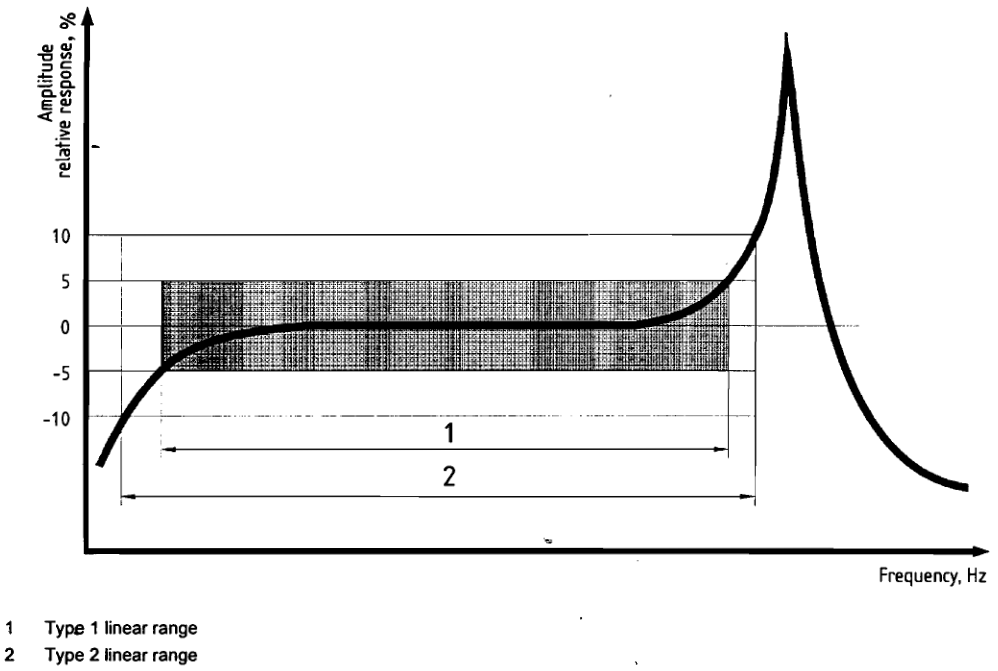
\includegraphics[width=0.8\textwidth]{assets/analysis/transducer-response.png}
	\caption{The transducer linear response and resonance in tolerance intervals~\cite{noauthor_iso_2002}}
	\label{fig:tranducer-response}
\end{figure}

Broadband measurement requires ``frequency ranges of 0.2 times the lowest rotational frequency to the highest frequency of interest''~\cite{noauthor_iso_2002}, not exceeding 10 kHz, with rms velocity 0.1 - 100~mm/s. Bearings and gear diagnosis may push the upper-frequency limit even higher. The tolerances of amplitude and frequency calibrations fall into two types with allowable tolerances of $\pm 5 \%$ or $\pm 10 \%$~(Fig.~\ref{fig:tranducer-response}).

Equipment's ``health'' can be mischaracterized when there are significant differences in the machine's normal operating conditions. Baseline measurements in all acceptable conditions are to be acquired to reduce the error in vibration evaluation. According to the bathtub curve~(Fig.~\ref{fig:bathtub-curve}) reference signatures should be obtained after the initial part wear-in period. The reference spectral mask of the baseline condition is designed if maximal acceptance amplitudes are different for each significant frequency band~\cite{ziaran_technicka_2013}.

The vibration baseline is defined by broad-band magnitudes and phases of motion vectors, the waveform in the time and frequency domain, the rotational speed of the machine as well as its frequency response to different speeds during start-up and coast-down captured in the Bode plot and waterfall plot. Changes during the machine's operation are then depicted in value trends. Trends can be shown by overall amplitudes or limited to frequency bands.

\section{Signal preprocessing} \label{section:signal-preprocessing}
The vibration signals in a factory environment are inherently full of disturbances. Nearby equipment operation and heavy objects handling in the surroundings can all contribute to the unwanted chaotic movement in otherwise mostly pure oscillatory motion. In addition, accelerometers suffer from systematic measurement errors in the form of thermal noise, zero-g offset from slight miscalibration, and bias originating from a constant force of gravity. These unavoidable distortions are somewhat suppressable by digital filters. In the preprocessing stage, we consider trend removal and time synchronous averaging to eliminate external interference.

\subsection{Detrending}
The oscillatory motion should be centered around the zero level for further manipulation. The constant offset is eliminated simply by subtracting the overall mean from the signal. Moreover, the high pass DC blocker infinite impulse response (IIR) filter of 1st order can adjust to shifts of the average value over time (Equation~\ref{equ:iir-dc-blocker}). The transition band depends upon the choice of corner frequency $f_{3dB}$ (Fig.~\ref{fig:dc-blocker}).

\myequations{DC blocker IIR filter of 1st order}
\begin{ceqn}\begin{align} \label{equ:iir-dc-blocker}
y_k = (1 - \frac{\omega}{2}) \cdot (x_k  -  x_{k - 1}) + (1 - \omega) \cdot y_{k - 1}; \quad \omega = 2\pi \cdot \frac{f_{3dB}}{f_s}
\end{align}\end{ceqn}

A steeper 3~dB attenuation band is achieved by increasing the order of the filter. Then, the cutoff frequency should be such that filter coefficients are fractions to counteract rounding errors~\cite{tittelbach-helmrich_digital_2021}.

\begin{figure}[h]
	\centering
	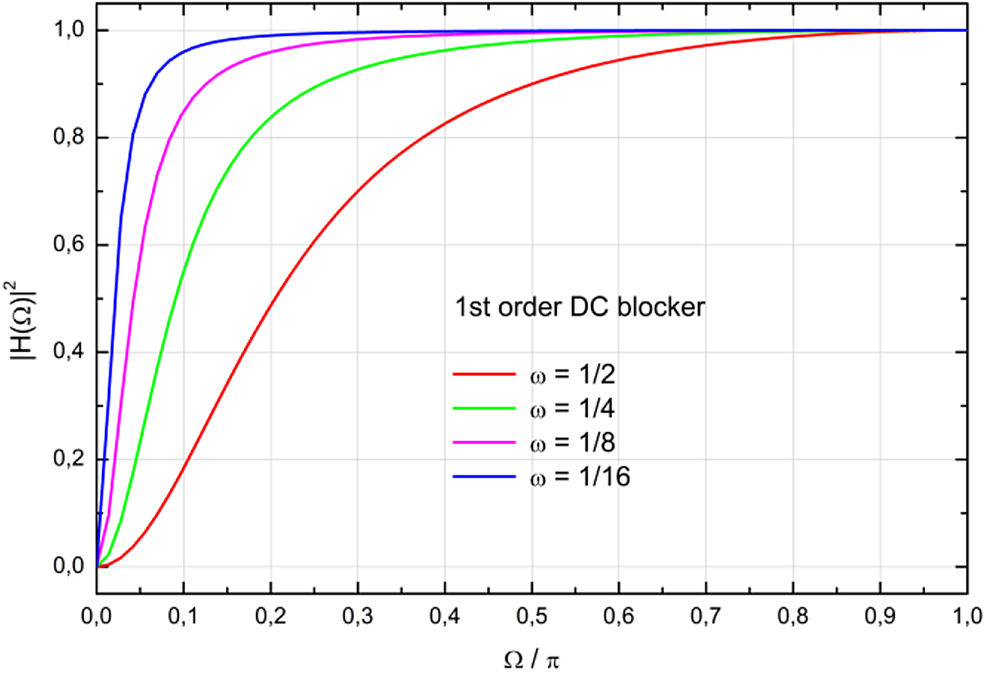
\includegraphics[width=0.7\textwidth]{assets/analysis/iir-1-dc-blocker-band.jpg}
	\caption{Transfer function of 1st order DC blocker filters ~\cite{tittelbach-helmrich_digital_2021}}
	\label{fig:dc-blocker}
\end{figure}

The finite impulse response (FIR) filter is not recommended for DC component removal because of the undesirable ripple effect with the small number of taps. Cascaded-integrator-comb (CIC) filters are proposed as an alternative instead~\cite{lyons_understanding_2011}.

\subsection{Time synchronous averaging}
Time synchronous averaging (TSA) diminishes the impact of vibration sources unrelated to the rotational frequency and its harmonics. TSA averages time-domain waveform over $N$ points and aligns it to a synchronization pulse with period $T$ (Equation~\ref{equ:tsa-average}).

\myequations{Time synchronous averaging}
\begin{ceqn}\begin{align}
x_{TSA} = \frac{1}{N} \sum_{n = 0}^{N - 1}{x(t + nT)}
\label{equ:tsa-average}
\end{align}\end{ceqn}

This technique has been successfully applied to the gearbox and bearing fault diagnosis~\cite{davies_handbook_2012,nandi_condition_2019}.

\section{Feature extraction} \label{section:feature-extraction}
After preprocessing, raw numerical vectors are merely low-level descriptors of the underlying physical phenomena. At first, these incomprehensible sequences of numbers are reduced to summary attributes called features in the process of feature extraction or feature discovery. Features can be hand-crafted (as is our case), learned implicitly within the model representation, or explicitly from an optimization problem solution.

Predictive maintenance has ideal prerequisites for the application of feature engineering because the signal is usually pseudo-stationary, and the trend monitoring variables come out of extensive domain expertise in mechanics. The advantages of the add-in extraction effort as opposed to processing unmodified samples are to gain better classification precision and reduce computational burden and storage capacity downstream with dimensionality reduction~\cite{johnson_feature_2019}.

It is important to note that the design of features is not a standalone step in the machine learning pipeline, but it should be performed iteratively to improve the target model. Signal features are computed in the time and frequency domain~\cite{brito_fault_2021}.

\subsection{Time-domain features}
The most widely found features in the literature are rudimentary statistical measures of the central moment: mean, variance, standard deviation, skewness, and kurtosis~(Tab.~\ref{tab:td-features}). Statistics can be calculated in any domain, but the mean value should not be used in detrended data. The vibration severity metrics out of technical standards are also highly regarded. The amplitude characteristics include root-mean-square and peak-to-peak distance~\cite{mostafavi_novel_2021}. The waveform shape is captured by zero-crossing rate and average amplitude change~\cite{moctar_time-domain_2023}.

The other significant time-domain attributes are derived as ratios of previous simpler ones. These ratios are crest, clearance, impulse factor, and shape factor~(Tab.~\ref{tab:td-features})~\cite{nandi_condition_2019}. Many articles have been successful in fault detection of bearings out of transients in impulsive signals with kurtosis, crest, and clearance factor~\cite{brito_fault_2021}. It is also suggested that the shape factor can signify unbalance and misalignment faults~\cite{nandi_condition_2019}.

\begin{table}[h]
\centering
\renewcommand{\arraystretch}{2}
\begin{tabular}{|l|l|l|l|}
\hline
\textbf{Feature}            & \textbf{Equation}                                                                    \\ \hline
\textit{Peak-to-peak}       & $ X_{ppv} = \max(x_i) - \min(x_i) $
\\ \hline
\textit{Zero-crossing rate} & $X_{zc} = \frac{1}{N}\sum_{i = 1}^{N}{\mathrm{sgn}(x_i \cdot x_{i-1})} $
\\ \hline
\textit{Root mean square}   & $ X_{rms} = \sqrt{\frac{1}{N}\sum_{i = 1}^{N}{x_i^2}} $
\\ \hline
\textit{Skewness}           & $ X_{sv} = \frac{1}{N}\sum_{i = 1}^{N}{\left(\frac{x_i - \bar{x}}{\sigma}\right)^3}$
\\ \hline
\textit{Kurtosis}           & $ X_{kv} = \frac{1}{N}\sum_{i = 1}^{N}{\left(\frac{x_i - \bar{x}}{\sigma}\right)^4}$
\\ \hline
\textit{Shape factor}   & $ X_{sf} = \frac{X_{rms}}{\frac{1}{N} \sum_{i=1}^{N}{|x_i|}}$
\\ \hline
\textit{Crest factor}   & $ X_{cf} = \frac{max(|x_i|)}{X_{rms}} $                           \\ \hline
\textit{Impulse factor} & $ X_{if} = \frac{max(|x_i|)}{\frac{1}{N} \sum_{i=1}^{N}{|x_i|}} $
\\ \hline
\textit{Clearance factor}  & $ X_{mf} = \frac{max(|x_i|)}{\left( \frac{1}{N} \sum_{i=1}^{N}{\sqrt{|x_i|}} \right)^2} $
\\ \hline
\textit{Average Amplitude Change (AAC)}        & $ X_{AAC} = \frac{1}{N}\sum_{i = 1}^{N - 1}{|x_{i + 1} - x_i|} $                             \\ \hline
\end{tabular}
\caption{Time-domain features}
\label{tab:td-features}
\end{table}


\subsection{Frequency-domain features}
The mechanical faults present themselves as oscillatory patterns which are combinations of frequencies with various amplitudes. The Fourier transform is one of the most prominent strategies in power spectral density estimation. Experts on vibrodiagnostics utilize it as a primary signal processing technique for data analysis as it is recommended in ISO 13373-2 standard~\cite{noauthor_iso_2016_2}.

The inherent symmetries in the Fourier matrix made it possible to implement the Fast Fourier transform (FFT) algorithm with time complexity $O(n \log n)$. The drawback of the plain spectral analysis is the lack of resolution for events that occurred at distant time instants, and so their spectral components might adversely blend in together.

\begin{table}[ht]
\renewcommand{\arraystretch}{2}
\centering
\begin{tabular}{|l|l|}
\hline
\textbf{Feature}           & \textbf{Equation}                                                                                                  \\ \hline
\textit{Spectral centroid} & $ X_{fc} = \frac{\sum_{i = 0}^{N - 1}{f_i \cdot a(f_i)}}{\sum_{i = 0}^{N - 1}{a(f_i)}}$                   \\ \hline
\textit{Energy}            & $ E(N) = \sum_{i = 1}^{N} a^2(t) $                                                                    \\ \hline \textit{Energy ratio}                & $E_r = E_i \;/\; \sum_{i = 1}^{N}{E_i} $                                                        \\ \hline
\textit{Spectral roll-on} & $ E(f_c) = 0.05 \cdot E(f_s / 2) $ \\ \hline
\textit{Spectral roll-off} & $ E(f_c) = 0.85 \cdot E(f_s / 2) $                                                   \\ \hline
\textit{Spectral flux}     & $X_{\mathrm{flux}} = 1 - \mathrm{corr}(A_{t-1}, A_t)$ \\ \hline
\textit{Noisiness}                   & $X_{noise} = \mathrm{SNR}(X) = \mu \;/\; \sigma $                             \\ \hline
\textit{Shannon entropy}      & $H(X) = - \sum_{i} P(X = x_i) \cdot \ln(P(X = x_i)) $                                                  \\ \hline
\textit{Spectral negentropy}      & $\Delta I_E(f, \Delta f) = \sum_{k = 0}^{N - 1}{p \cdot \ln(p); p = \frac{\mathrm{SES}^2}{\frac{1}{N} \sum_{k=0}^{N-1} \mathrm{SES}^2}}$                                                \\ \hline
\end{tabular}
\caption{Frequency-domain features}
\label{tab:fd-features}
\end{table}

In the frequency domain, we can obtain the usual statistical properties of the distribution which are spectral centroid, skew, and kurtosis. Additionally, spectral roll-on and roll-off, fundamental frequency, entropy, negentropy, spectral flux, signal-to-noise ratio (noisiness), energy in frequency bands, and energy ratio are extracted (Tab.~\ref{tab:fd-features})~\cite{peeters_large_2004}.

In geometric terms, the spectral centroid represents the barycenter of the frequency magnitude plot. Spectral roll-off gives a notion about the spectral distribution because it identifies the frequency $f_c$ below which 85\% of the signal energy is contained. The roll-on frequency is chosen so that 5\% of the signal energy is below this value. According to the definition, spectral flux is normalized cross-correlation between two successive amplitude spectra. A flux value of one means the spectra are the most dissimilar.

``Negentropy measures the inclination of a system to increase its level of organization''~\cite{avoci_spectral_2020}. The larger \emph{spectral negentropy} suggests more fault-induced impulses. The squared envelope spectrum (SES) is interpreted as $E(k, f, \Delta f)$ which is an envelope in the Fourier domain: $\mathcal{F}\{ |y(k, f, \Delta f)|^2 \}$.

\subsection{Features in harmonic frequencies}
If a single principal frequency exists, it can be determined by maximum likelihood estimation. Such frequency would explain the signal spectrum the best~\cite{peeters_large_2004}. The frequency spectrum is a discrete set of amplitudes where peaks have to be reliably identified to create representative attributes.

The essential peak-finding approaches are based either on magnitude or gradient. All found extrema are commonly filtered with the magnitude of prominences and the width at half prominence. In the magnitude-based method, the middle point $x_i$ is compared to two neighbouring points and the peak is then: $x_{i-1} < x_i > x_{i+1}$. The gradient-based method evaluates the first derivative at the point that is equal to zero if the point is a local maximum, local minimum, or inflection point~\cite{adikaram_non-parametric_2016}.

A substantial improvement is a robust non-parametric peak identification named \emph{MMS} based on the sum of terms in an arithmetic progression based on maximum, minimum, and sum. MMS max-min finder in the elementary form processes points in the window of length 3, it advances one point and deems its middle point as a local extremum if it satisfies equalities below. Equation~\ref{equ:mms-maxima} is for the hill and Equation~\ref{equ:mms-minima} is for the valley. The filtration techniques are incorporated in the adaptations of the MMS algorithm: MMS-WBF, MMS-SG, MMS-LH~\cite{adikaram_non-parametric_2016}.

\myequations{MMS algorithm: Local maxima identification equality}
\begin{ceqn}\begin{align}
\frac{a_{max} - a_{min}}{S_3 - a_{min} \cdot 3} = \frac{a_{mid} - a_{min}}{S_3 - a_{min} \cdot 3}
\label{equ:mms-maxima}
\end{align}\end{ceqn}

\myequations{MMS algorithm: Local minima identification equality}
\begin{ceqn}\begin{align}
\frac{a_{max} - a_{min}}{a_{max} \cdot 3 - S_3} = \frac{a_{max} - a_{mid}}{a_{max} \cdot 3 - S_3}
\label{equ:mms-minima}
 \end{align}\end{ceqn}

\myequations{Harmonic series search criterion}
\begin{ceqn}\begin{align}
v_i^{(r)} = \frac{v_j}{\min{|v_j - r \cdot v_i|}}
\label{equ:harmonic-search}
\end{align}\end{ceqn}

Multiple harmonic series and the sidebands can be separated into a discrete set of frequency components, each with a central frequency, uncertainty, and amplitude $C_i(v_i, \Delta v_i, A_i)$ by an exhaustive search algorithm. Harmonic family identification is a non-trivial problem because of spectrum estimation errors. The criterion is proposed to select harmonics at the minimal distance from the true fundamental frequency multiple~(Equation~\ref{equ:harmonic-search}). Two series with the same fundamental frequency are merged and thought of as a modulation series~\cite{gerber_identification_2013}.

\subsection{Time-frequency domain features}
The \textbf{Short-time Fourier transform} (STFT) splits the time-domain signal into equal-length intervals. Individual chunks have a 50\% overlap and are multiplied with weights of window function to balance scalloping loss and spectral leakage due to the Fourier transform periodicity assumption. Traditionally, the Hann window is commonly used instead of the rectangular window~\cite{ziaran_technicka_2013,noauthor_iso_2016_2}.

In the time-frequency domain, the same features can be derived as in the frequency domain, but in addition, the attributes are time-localized in this way. The STFT has a considerable flaw for implementation in a self-adaptable system and that is fixed resolution. The optimal window size has to be set beforehand or chosen after performing multiple transformations on chunks out of the range of lengths. Welch's method averages multiple consecutive blocks to better estimate the spectrum. We have already researched the suitability of STFT for online detection of constant frequencies~\cite{hajek_iot_2022}.

The alternative to isolating weak impacts with high time resolution is a \textbf{Teager-Kaiser energy operator} (TKEO) (Equation~ \ref{equ:tkeo-operator}). It is a tool for envelope analysis to demodulate characteristic AM-FM signals present during bearing faults. Energy operator output can be utilized as a standalone feature attribute.

\myequations{Teager–Kaiser energy operator}
\begin{ceqn}\begin{align}
\psi[x(n)] = [x(n)]^2 - x(n - 1)x(n + 1)
\label{equ:tkeo-operator}
\end{align}\end{ceqn}

Improved TKEO is necessary to prevent analysis from suffering from the noisy source. The key idea is to perform TKEO after signal decomposition into narrowband components with different center frequencies. The extracted modes are reconstructed with weights assigned based on their correlations to the original signal~\cite{shi_application_2022}.

Time-frequency spectrum modification preserving localization of abrupt wideband spikes at time $t_0$ and simultaneously reducing energy smear over the larger region is a goal of \textbf{Transient-extracting transform} (TET). Post-processing of STFT window $G(t,\omega)$ involves multiplication of the spectrum with the Transient extracting operator (TEO). This operator is expressed in the form of a Dirac delta function $\delta(t)$ (Equation~\ref{equ:tet-transform}).

\myequations{Transient-extracting transform}
\begin{ceqn}\begin{align}
\mathrm{Te}(t,\omega) = G(t,\omega) \cdot  \delta(t - t_0)
\label{equ:tet-transform}
\end{align}\end{ceqn}

TET representation retains non-zero coefficients where the absolute value of the ratio between two STFTs, $G^{tg}[n, k]\;/\;G[n, k]$ is less than half the sampling interval $T$. These two transforms use distinct windows $g[n]$ and $n \cdot g[n]$. Decomposition of a signal with TET is proved to produce significantly larger kurtosis (around 38 in TET, 4 in other methods) and hence better discriminate the transient fault~\cite{yu_concentrated_2020}.

\subsection{Wavelet domain features}
The bands for lower frequencies should be longer in time than for higher frequencies. The \textbf{Wavelet transform} (WT) possesses such a multiscale discrimination property, effectively increasing resolution in time-frequency plain. Wavelet basis functions are constructed for that purpose (Equation~\ref{equ:mother-wavelet}). There are several wavelet families. For example, Haar, Daubechies, Coiflets, Symlets, Morlet, and Meyer~\cite{nandi_condition_2019}.

\myequations{Mother wavelet function}
\begin{ceqn}\begin{align}
\psi_{s, \tau} = \frac{1}{\sqrt{s}}\psi\left(\frac{t - \tau}{s}\right)
\label{equ:mother-wavelet}
\end{align}\end{ceqn}

\textbf{Continuous Wavelet transform} (CWT)~(Equation~\ref{equ:cwt-transform}) is done by scaling and translating the mother wavelet $\psi$ picked out of the appropriate family~\cite{nandi_condition_2019}. The scale factor is denoted with~$s$ and time position with~$\tau$. The choice of wavelet type is data-driven because distinct wavelet shapes have an impact on the response and ultimately contribute to filter length. The decision lies between recognition abilities for impulse-like signals or the inclusion of wider surrounding space.

\myequations{Continuous Wavelet transform}
\begin{ceqn}\begin{align}
W_{x(t)}(s, \tau) = \frac{1}{\sqrt{s}}\int x(t) \cdot \psi^*\left(\frac{t - \tau}{s}\right)\;\mathrm{dt}
\label{equ:cwt-transform}
\end{align}\end{ceqn}

The CWT is computationally intensive when a highly detailed scale resolution is required because each wavelet scale convolves with the entire signal. The fCWT algorithm allows 100 times higher spectral resolution than previous implementations at the same speed. It increases performance 122 times compared to Wavelib and 34 times in comparison with PyWavelets~\cite{arts_fast_2022}.

The fast CWT algorithm reaches compelling improvement by applying Parseval's theorem to the wavelet transform formula that removes the dependence on the time offset parameter~\cite{arts_fast_2022}. The convolution takes place with the mother wavelet in the Fourier base. Then, the inverse FFT produces the coefficients for individual scales.

\textbf{Synchrosqueezing Wavelet transform} (SST) is a modification of CWT attempting to sharpen the representation of frequency components by coefficient reassignments from around the central frequencies towards the middle of the bands. The justification for these reallocations is rooted in the signal approximation as amplitude-modulated oscillating modes with additive noise $\eta(t)$ (Equation~\ref{equ:sst-transform})~\cite{herrera_applications_2014}.

\myequations{Representation of components for Synchrosqueezing Wavelet transform}
\begin{ceqn}\begin{align}
s(t) = \sum_{k=1}^{K} A_k(t)\cos(\theta_k(t)) + \eta(t)
\label{equ:sst-transform}
\end{align}\end{ceqn}

The components are defined by their instantaneous amplitudes $A_k(t)$ and instantaneous phases $\theta_k(t)$. The energy spread to adjacent bins can be effectively squeezed only in regions with constant phase and large enough component separation. Despite the promising properties of this transform, white noise causes severe interference in the resulting time-frequency map.

The spectrograms to illustrate the difference in the ability of the Fourier transform, the continuous Wavelet transform, and their modifications to pick up underlying patterns in bearing faults are shown in Fig.~\ref{fig:transforms}.

\begin{figure}[ht]
    \centering
    \begin{subfigure}[b]{0.49\textwidth}
        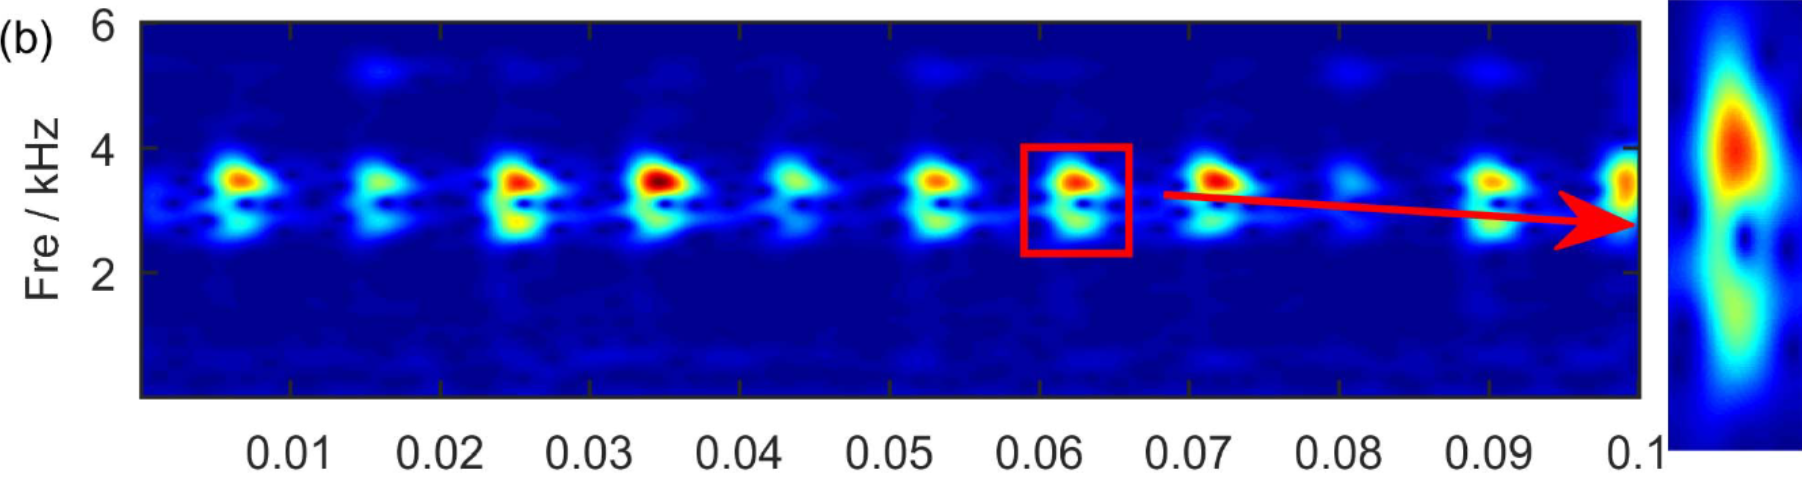
\includegraphics[width=\textwidth]{assets/analysis/stft-spectrogram-sample.png}
        \caption{STFT \& Gaussian window}
    \end{subfigure}
    \hfill
    \begin{subfigure}[b]{0.49\textwidth}
        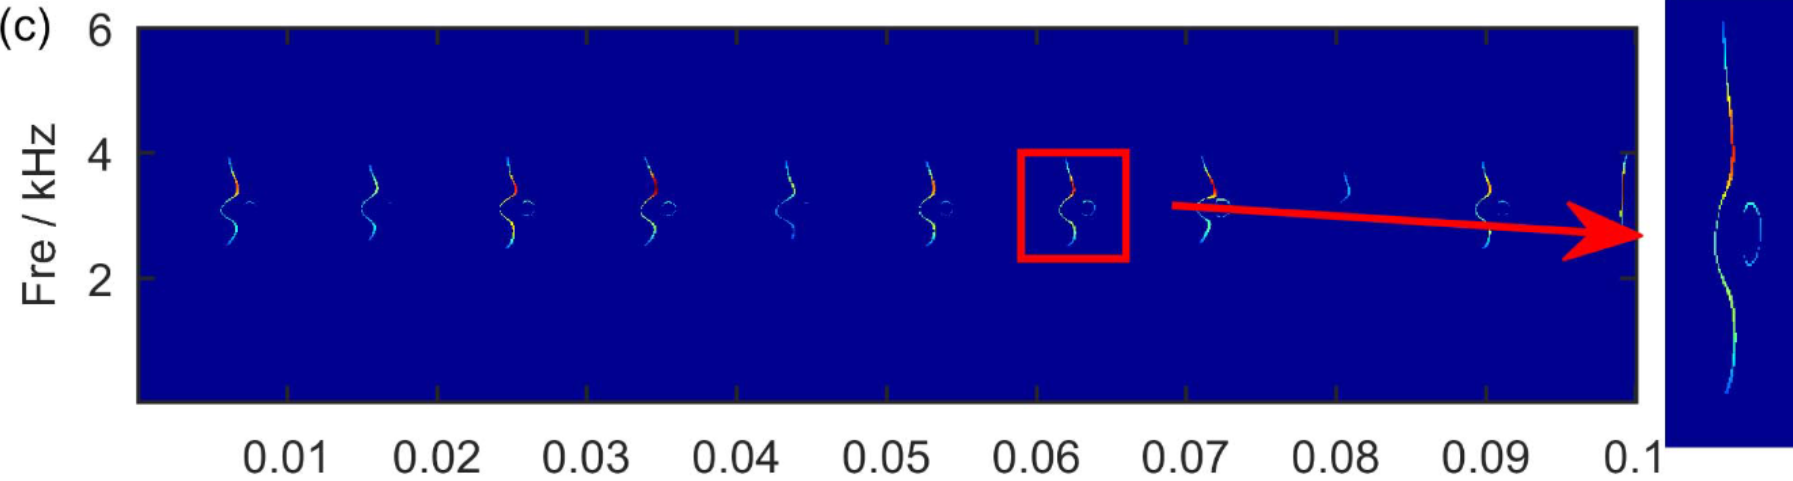
\includegraphics[width=\textwidth]{assets/analysis/tet-spectrogram-sample.png}
        \caption{TET}
    \end{subfigure}
    \hfill
    \begin{subfigure}[b]{0.49\textwidth}
        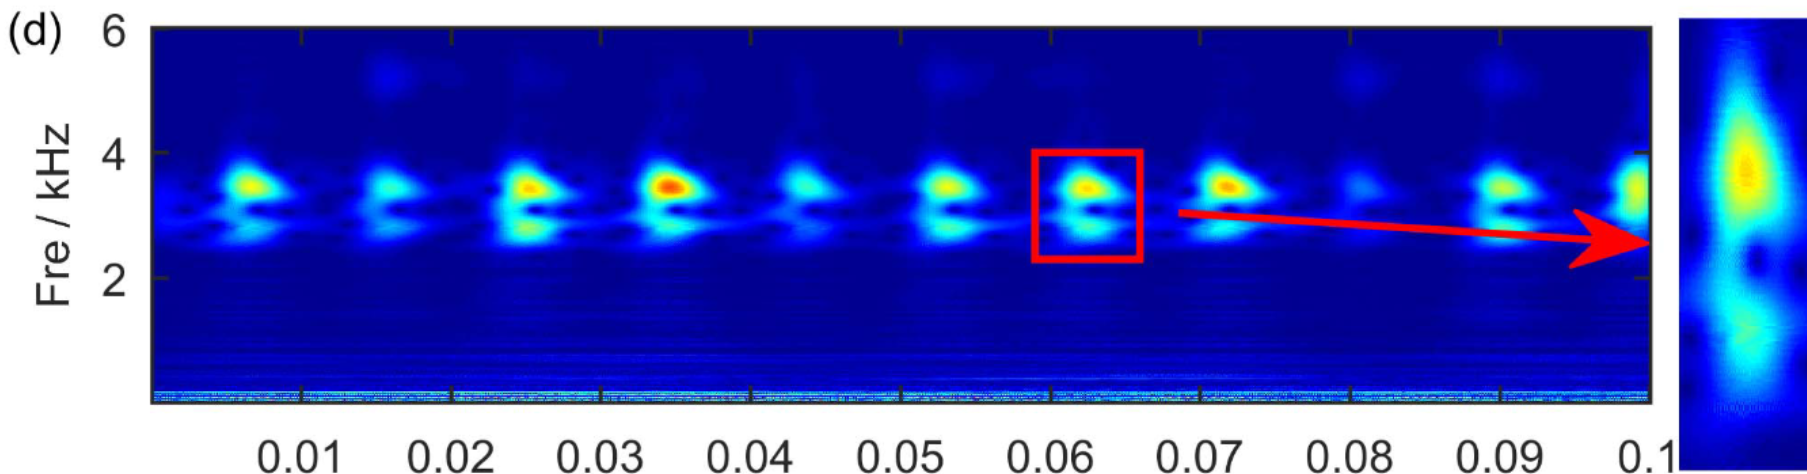
\includegraphics[width=\textwidth]{assets/analysis/wt-spectrogram-sample.png}
        \caption{CWT \& Morlet wavelet}
    \end{subfigure}
    \hfill
    \begin{subfigure}[b]{0.49\textwidth}
        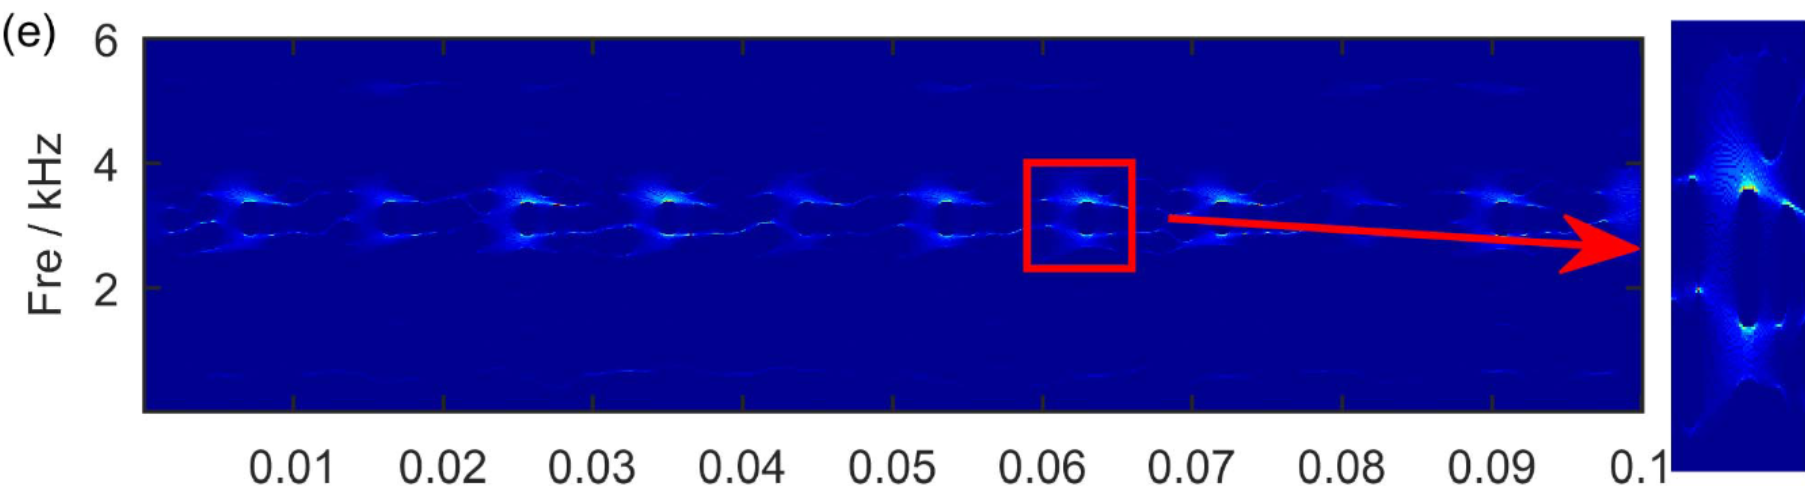
\includegraphics[width=\textwidth]{assets/analysis/sst-spectrogram-sample.png}
        \caption{SST}
    \end{subfigure}
    \caption{Comparison of time-frequency transform spectrograms~\cite{yu_concentrated_2020}}
    \label{fig:transforms}
\end{figure}

The dyadic filter bank is another signal decomposition technique that generates subbands at multiple granularity levels. The practical realization of the multiscale description is \textbf{Discrete Wavelet Transform} (DWT). The DWT behaves as a quadrature mirror filter and splits waveforms using a wavelet filter to detail coefficients (D1) and approximation coefficients (A1) (Fig.~\ref{fig:dwt-filter-bank})~\cite{nandi_condition_2019}. The low-pass filter $h(k)$ creates approximation coefficients further decomposed at the successive levels. Detail coefficients represent the result of the high-pass filter $g(k) = (-1)^k h(1 - k)$ after decimation by a factor of 2.

The maximum depth of the decomposition tree is $\log_2{n}$ where $n$ is the number of input samples. Energy, energy ratio, and entropy are prevalent features that succinctly encode the wavelet coefficients. Otherwise, the additional extracted levels raise the total number of data dimensions.

In washing machine status classification, the discrete wavelet transform with Daubechies wavelet (db4) and fifth-level decomposition provides features with a combination of approximation (cA5) and detail coefficients (cD1, \dots, cD5). Washing machines belong to three categories: no fault, electric motor clamping screws problem, and a loose or broken counterweight. Extracted measures were sample mean and sample variances over autocorrelation functions of coefficients (AcD$n$) and smoothed coefficients cD1, cD2 by moving average filter~\cite{goumas_classification_2002}.

\textbf{Wavelet Packet Decomposition} (WPD) applies filters to split detail coefficients identically as approximation ones (Fig.~\ref{fig:wpd-filter-bank}) thus increasing the resolution in the high-frequency bands and providing uniform spectrum partitioning.

\myequations{Wavelet packet coefficient}
\begin{ceqn}\begin{align}
 w_{j,n,k} = \langle f, W_{j,k}^n\rangle = \langle f, 2^{j/2} W^n (2^jt-k) \rangle
\label{equ:wavelet-packet-coefficient}
\end{align}\end{ceqn}

Each wavelet packet coefficient $w_{j,n,k}$ captures subband frequency content around time instant $2^j k$ (Equation~\ref{equ:wavelet-packet-coefficient})~\cite{yen_wavelet_2000}. This measure is an inner product of the source and scaled wavelet packet function. The aforementioned feature extraction established in DWT can be applied. For example calculation of the wavelet packet node energy.

\begin{figure}[ht]
    \centering
    \begin{subfigure}[b]{0.49\textwidth}
        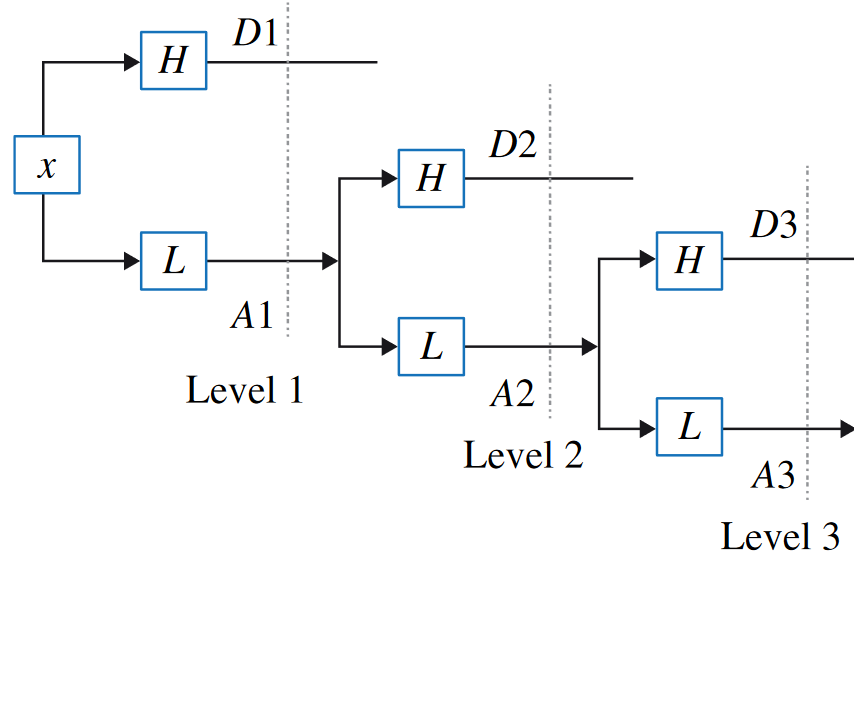
\includegraphics[width=\textwidth]{assets/analysis/DWT.png}
        \caption{Discrete wavelet transform}
        \label{fig:dwt-filter-bank}
    \end{subfigure}
    \hfill
    \begin{subfigure}[b]{0.49\textwidth}
        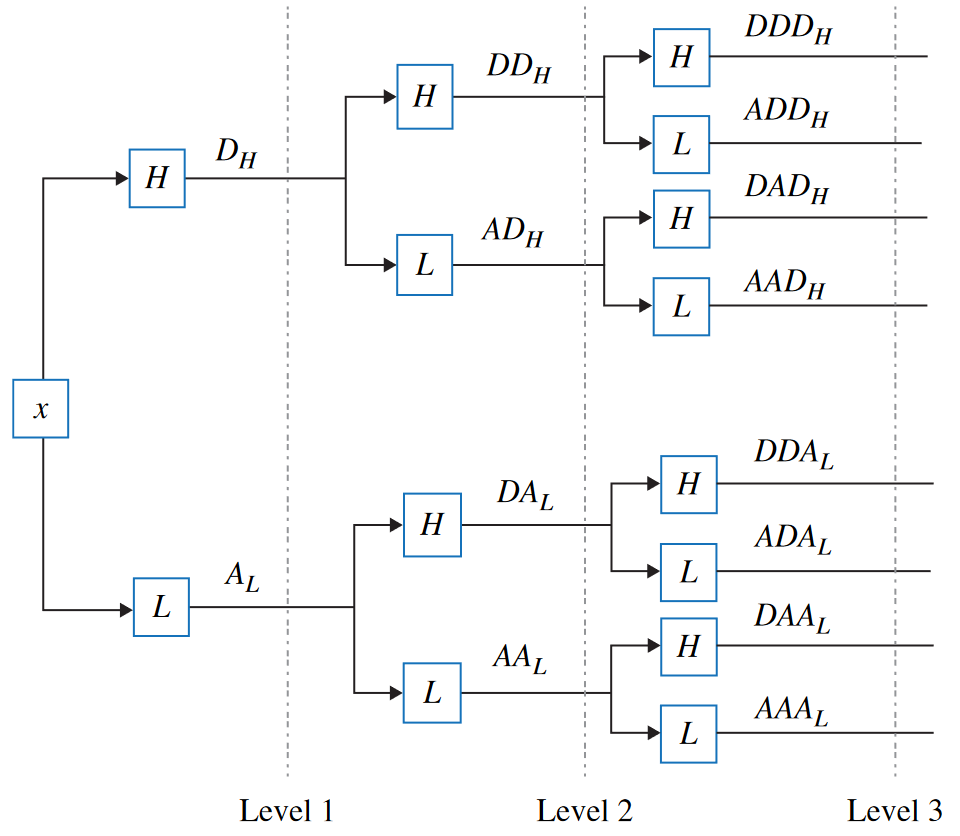
\includegraphics[width=\textwidth]{assets/analysis/WPD.png}
        \caption{Wavelet packet decomposition}
        \label{fig:wpd-filter-bank}
    \end{subfigure}
    \caption{Dyadic filter banks for discrete wavelet transform~\cite{nandi_condition_2019}}
\end{figure}

The wavelet packet energy ratio for weak feature extraction has been incorporated into the method of multiple frequency band demodulation (MFBD). The highest $n$ energy coefficients are selected out of 8 narrow frequency bands to subsequently affect the principal components. Demodulation principle for the frequency bandwidth prescribes $n$ to satisfy condition: $1\;/\;2^n > f_{\mathrm{modulation}}\;/\;f_s$. The first few eigenvectors that explain together more than 80\% of energy are retained to reconstruct the signal with a Fourier transform and retain the weak fault components~\cite{song_mfbd_2021}.

Tool wear diagnosis based on acoustic emission (AE) signal considers \emph{wavelet packet energy} in bands $E_{8}$, $E_{10}$, $E_{12}$, \emph{energy ratios} $P_{8}$, $P_{13}$, and \emph{energy entropy} as having high correlation ($|r| > 0.8$) with the band saw flank face width. The acoustic signal is decomposed into three layers using Daubechies db3 wavelet. The bottom layer contains bands numbered 7 through 14, each with a bandwidth of 62.5 kHz, because of the 1 MHz sampling frequency. The feature vector constructed in the article includes other statistical metrics out of power spectral density that have reached a notable correlation with evolving wear. The statistics are \emph{skewness}, \emph{kurtosis}, \emph{shape factor}, and \emph{centroid frequency}~\cite{zhuo_research_2022}.

Discrete wavelet transform and wavelet packets partition the spectrum into predefined frequency bands that do not always adequately capture individual elementary oscillations. Adaptive spectral segmentation is needed to extract separate intrinsic mode functions (IMF).

Wavelet domain features and associated spectral segmentation appear to be a powerful tool for conserving data bandwidth. These variables turn out to be difficult to communicate and comprehend. Therefore, we further use more standardized metrics.

\section{Feature transformations} \label{section:feature-selection}
Numerical features from the feature extraction phase have non-normal distributions and span wide ranges. Broad differences among features skew the spread on a particular axis. Inevitably, it can degrade the discernment of fault diagnostics models that map input onto a smooth function as regression does~\cite{zheng_feature_2018}. The feature scaling, power transform, and principal component analysis modify attribute values to gain more meaningful predictors, but one must be cautious in model interpretation.

\subsection{Feature normalization}
Vibrations are measured with an accelerometer in the form of 3D vectors where each axis has its own component. Models have to be resilient to any slight inclination or sensor orientation. To satisfy this prerequisite, feature $f$ extracted from all three dimensions is first composed into a single vector and the Euclidian norm is computed~\cite{kamminga_robust_2018}.

\myequations{Feature euclidian norm}
\begin{ceqn}\begin{align}
\widetilde{f} = \sqrt{f_x^2 + f_y^2 + f_z^2}
\end{align}\end{ceqn}

Feature normalization most often takes two forms. \textbf{Min-max scaling} changes the original range of values into an interval $[0, 1]$ (Equation~\ref{equ:min-max-scaler}). \textbf{Standardization} (Equation~\ref{equ:standardization-scaler}) constrains the mean of the variable to 0 with a variance of 1~\cite{zheng_feature_2018}.

\myequations{Min-max feature scaling}
\begin{ceqn}\begin{align}
\widetilde{x} = \frac{x - \min(x)}{\max(x) - \min(x)}
\label{equ:min-max-scaler}
\end{align}\end{ceqn}

\myequations{Feature standardization}
\begin{ceqn}\begin{align}
\widetilde{x} = \frac{x - \bar{x}}{\sigma_x}
\label{equ:standardization-scaler}
\end{align}\end{ceqn}


\subsection{Principal components analysis}
Highly correlated features generated from a relatively small original column space are redundant as they do not provide any additional information for diagnostics. \textbf{Principal Component Analysis} (PCA) solves this problem by projecting potentially linearly dependent features into a new feature space where the incoming information is preserved in a smaller number of features~\cite{zheng_feature_2018}. The threshold of how many principal components are picked depends on the amount of explained variance and desired quantity of data reduction.

\myequations{Singular Value Decomposition}
\begin{ceqn}\begin{align}
\mathbf{C} = \mathbf{U \Sigma V^T}
\label{equ:svd}
\end{align}\end{ceqn}

PCA consists of taking the Singular Value Decomposition (SVD) (Equation~\ref{equ:svd}) of the mean-centered input matrix. The disadvantage of this method is the loss of explainability in transformed space though it generally outperforms the model working with hand-crafted features~\cite{brito_fault_2021}. The signal samples can be processed directly by PCA without going through an intermediate step of calculating statistical measures.

\section{Feature selection}
Features do not contribute to the predictive power of the model with an even share. A certain subset can achieve better results than others. Choosing the optimal feature subset is the NP-hard combinatorial problem.

\subsection{Filtering methods}
The features can be chosen intrinsically as a part of a model by \emph{embedded methods} or by machine learning search algorithm at a serious computational expense in \emph{wrapper methods}. However, we will focus on \emph{filtering methods} which rank the predictors in order of their importance for the problem at hand and separate the best performing group~\cite{johnson_feature_2019}. The most common strategy is \emph{K-Best Selection}.

The general steps in selecting the appropriate predictors are as follows~\cite{nandi_condition_2019}:

\begin{enumerate}
    \itemsep0pt
    \item \textbf{Subset generation} - sets of features are generated in different search directions and with various strategies. Attributes are either appended to an empty set or pruned away from a universal set, sequentially or randomly.

    \item \textbf{Subset evaluation} - comparison of subset quality is assessed with relevance measures, some of which are discussed below.

    \item \textbf{Stopping criteria} - search is exhausted when the specified number of features has been found, subset metrics cannot be improved further, or satisfactory model performance is achieved. Subset generation and evaluation can be performed multiple times until the stopping criteria are met.

    \item \textbf{Validation} - the resulting subset is tested for the specific model on synthetic and real-world datasets against well-known results.
\end{enumerate}

Filter-based feature selection is preprocessing step independent of model choice with small computational requirements. Measures of information, correlation, similarity, and interdependence output the relevancy rating. Predictors are rated individually or in interacting congregations.

\subsection{Feature importance ranking}
Most of the scores are based on supervised learning, so they expect true class labels to apportion the measurements respectively. After the scores are assigned to the first $n$ features, those below a threshold are removed.

The frequently used scores upon which the feature relevance is ordered are~\cite{nandi_condition_2019}:

\begin{itemize}
\item \textbf{Variance threshold} - removes low-variance features below the set threshold.

\item \textbf{Correlation coefficient} - expresses the linear relationship between two variables. The codependent variables are of three sorts: quantitative, ordinal, and nominal. The choice of coefficient calculation is determined by the type of variables under consideration as shown in Table \ref{tab:corr-coef}.


\emph{Pearson correlation} coeficient expresses similarity between two quantitative features: $f_i$ and $f_j$. In the classification setting, the correlation of feature $f$ makes sense only with dichotomous target class label $c$ using \emph{point biserial coeficient}. Mathematically, this is equivalent to the Pearson coefficient. Rank correspondence is quantified with either Spearman rho or Kendall's Tau~\cite{calkins_more_2005}.

\begin{table}[ht]
\renewcommand{\arraystretch}{1.5}
\begin{adjustbox}{width=\columnwidth,center}
\begin{tabular}{|c|l|l|l|}
\hline
\textbf{Variable Y\textbackslash{}X} & \multicolumn{1}{c|}{\textbf{Quantitiative X}} & \multicolumn{1}{c|}{\textbf{Ordinal X}} & \multicolumn{1}{c|}{\textbf{Nominal X}} \\ \hline
\textbf{Quantitative Y}              & Pearson $r$                                   & Biserial $r_b$                          & Point Biserial $r_{pb}$                 \\ \hline
\textbf{Ordinal Y}                   & Biserial $r_b$                                & Spearman $\rho$    & Rank Biserial $r_{rb}$                  \\ \hline
\textbf{Nominal Y}                   & Point Biserial $r_{pb}$                       & Rank Bisereal $r_{rb}$                  & Phi, L, C, Lambda                       \\ \hline
\end{tabular}
\end{adjustbox}
\caption{Correlation coeficients}
\label{tab:corr-coef}
\end{table}

Attributes are ranked in descending order according to the absolute value of their correlation coefficient. We seek the highest correlation to the class label.

\myequations{Pearson correlation coefficient}
\begin{ceqn}\begin{align}
r(i) = \frac{\mathrm{cov}(f, c)}{\sqrt{\mathrm{var}(f) \cdot \mathrm{var}(c)}}
\end{align}\end{ceqn}


\item \textbf{Fisher score} - measures the difference between the means of the classes. It is interchangeable with ANOVA F-value, but it is evaluated for each feature $X^j$ separately. Ideally, the features in the subset have large distances between samples of various classes in $C$ and distances within a class are the smallest possible. In the formula (\ref{equ:fisher-score}), $n_j$ is the sample size of $j$th feature, $\mu^j$ is its sample mean, and $\mu$ is the overall mean.

\myequations{Fisher score}
\begin{ceqn}\begin{align}
\mathrm{FS}(X^j) = \frac{\sum_{i=1}^{C} n_i(\mu_i^j - \mu^i)^2}{\sum_{i=1}^{C} (n_i - 1) \cdot (\sigma_i^j)^2}
\label{equ:fisher-score}
\end{align}\end{ceqn}

\item \textbf{Mutal information} - quantifies the dependence between features, or between features and class labels. It is almost identical to Information Gain. The probability distribution of proximity of variables derives from the relative entropy known as the Kullback-Leibler distance. Mutual information presumes variables are discrete. In the case of quantitative variables, mutual information is estimated by binning or nearest neighbours methods~\cite{ross_mutual_2014}.

Probabilities $P(x)$, $P(y)$, $P(x, y)$ are estimated in the contingency table from event occurrence count to all sample population $|x|\;/\;N$. Joint probability $P(x, y)$ represents samples of feature $x$ simultaneously in class $y$.

\myequations{Mutal information}
\begin{ceqn}\begin{align}
\mathrm{MI}(X, Y) = \sum_{y \in Y} \sum_{x \in X} P(x, y) \cdot \log\left(\frac{P(x, y)}{P(x)P(y)}\right)
\end{align}\end{ceqn}
\end{itemize}

Multiple subsets of predictors produced by each evaluation metric can train several variants of a classification model. Sets of attributes can be combined into an ensemble by \emph{electoral system}. One such example is \textbf{majority voting} which chooses the best feature out of the group. \textbf{Rank product} unifies several feature orderings by computing the geometric mean of feature rank in every experiment realization~\cite{breitling_rank_2004}.

\section{Diagnostics techniques} \label{section:diagnostics-techniques}
Fault identification in the rotating machinery is a one-class or multi-class classification problem acting in a semi-supervised manner because labels for degraded conditions are scarce in practice. The automation goals in monitoring can be broadly categorized as anomaly detection and recognizing the momentary fault type.

The guiding principles for algorithm selection are simplicity in terms of their straightforward visual explanation for the production managers, and the ability to progressively improve the model on the streaming data to address peculiarities in individual machine constructions.

\subsection{Novelty detection}
Anomaly, novelty, or outlier detection determines whether a health status deviates considerably from the baseline profile. The expert can then step in and diagnose the machine after the notice. Anomaly is a rare observation different from the others, raising suspicion that it was created by unrelated behavior~\cite{aggarwal_outlier_2016}. The observations get assigned anomaly scores, and those over the threshold are novelties.

The measurements coming in the steaming fashion have to be processed in a single pass. The detection model must deal with the minimal admissible assumptions about the nature of the input events. The outliers are derived based on non-parametric statistical models, nearest-neighbour clustering, and isolation-based approaches~\cite{gervasi_anomaly_2020}.
\bigbreak

\textbf{DenStream} is a density-based algorithm adapted from DBSCAN to cluster streaming data of arbitrarily shaped groups. Samples it includes in the first step into coherent clusters are core data points in each other's neighbourhoods. Core points have at least \emph{MinPts} ($\mu$) points in their neighbourhood of radius \emph{Eps} ($\varepsilon$) units. Then non-core points in the proximity area of the core point are attached to the cluster containing it~\cite{aggarwal_data_2014}.

Quality of clustering results is evaluated by \emph{Silhouette score} in the range [-1; 1]. It demands points within clusters to have high cohesion and at the same time to have large separation from other clusters. The low score indicates a too-small or too-large number of clusters~\cite{rousseeuw_rousseeuw_1987}.

\begin{figure}[ht]
    \centering
    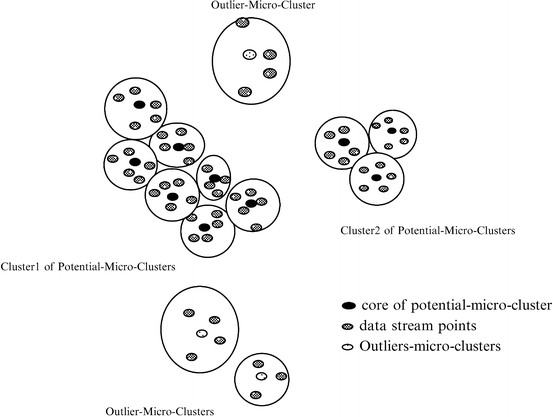
\includegraphics[width=0.8\textwidth]{assets/analysis/DenStream.png}
    \caption{DenStream~\cite{amini_density_2012}}
    \label{fig:denstream}
\end{figure}

In the online maintenance phase, DenStream summarizes the nearby observations into core \emph{micro-clusters} that can be potential micro-clusters or outlier \emph{micro-clusters} (Fig.~\ref{fig:denstream})~\cite{ghesmoune_state---art_2016}. The (outlier) \emph{o-micro-clusters} can grow into (potential) \emph{p-micro-clusters} when they encompass $\beta \mu$ points. The outliers are discounted after some time in accordance with the decay function: $f(t) = 2^{-\lambda t}$ or below the lower weight limit $\xi$. The on-demand offline stage runs DBSCAN over the approximate representation in micro-clusters to deliver final apportionment~\cite{cao_density-based_2006}.

\subsection{Classification}
Accurate multi-class classification of machine faults according to the characteristics of known causes is a much more difficult task than novelty detection. Fault combinations have to be recorded and transformed into feature space. Interactions among fault root causes have to be considered. We are aware of rapid advances in knowledge transfer for deep neural networks~\cite{maurya_condition-based_2021}. So far, solutions seem to be hard to implement. Therefore, we opt to use a simpler model.

The performance of classification is estimated by several metrics on the validation set obtained using hold-out or cross-validation techniques. Frequently used quantities for classifier model evaluation include accuracy, precision, recall, f1 score, area under the ROC curve, and counts of hits and misses in a confusion matrix.
\bigbreak

\textbf{K-nearest neighbours} (k-NN) assigns the data point to the class where the majority of $k$ closest instances belong (Fig.~\ref{fig:KNN}). It means it can work in a semi-supervised environment because it can infer labels just from knowing a few annotations. The major drawback of k-NN is a preference for the majority class in imbalanced class-size datasets. The issue is mitigated with class weights or resampling classes by oversampling or undersampling. The model without class balancing drops in precision from 15\% to over 40\% depending on the imbalance ratio~\cite{shi_improving_2020}. The k-NN algorithm requires features to be normalized to assign the same importance to each predictor.

\begin{figure}[ht]
    \centering
    \begin{subfigure}[b]{0.49\textwidth}
        \includegraphics[width=\textwidth]{assets/analysis/KNN.png}
        \caption{k-NN with k = 5}
        \label{fig:KNN}
    \end{subfigure}
    \hfill
    \begin{subfigure}[b]{0.49\textwidth}
        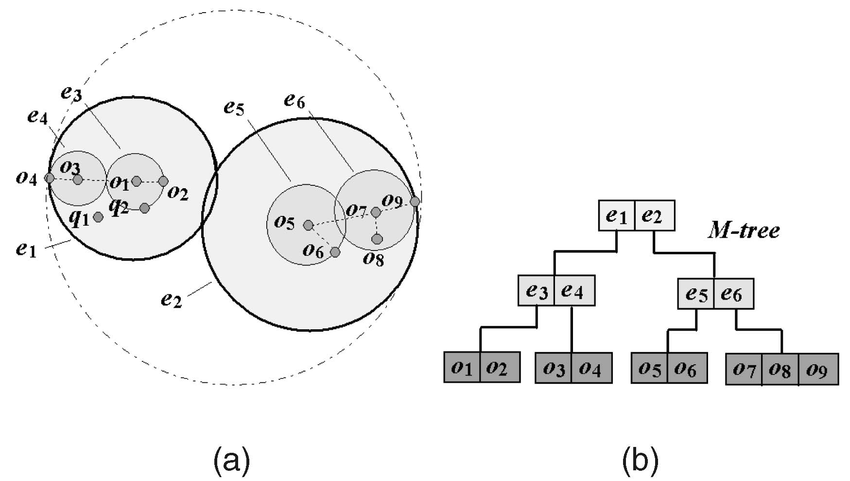
\includegraphics[width=\textwidth]{assets/analysis/M-tree.png}
        \caption{M-tree data structure}
        \label{fig:m-tree}
    \end{subfigure}
    \caption{Nearest neighbours classification algorithm~\cite{chen_skyline_2009}}
\end{figure}

The meaning of distance between feature vectors $\mathbf{x}$, $\mathbf{y}$ have to be defined, so several metrics are available like \emph{Euclidian distance}, \emph{Mahalanobis distance}, \emph{Manhatann distance} etc. (Tab.~\ref{tab:KNN-distance})~\cite{sheng_review_2020, abu_alfeilat_effects_2019}. The optimal $k$ parameter is set by supervised learning according to the breaking point in the elbow curve that plots choices of $k$ against the error rate. The demanding neighbourhood queries are sped up using spatial indexes in databases that utilize search trees such as kd-tree, R-tree, or M-tree.

\begin{table}[ht]
\centering
\renewcommand{\arraystretch}{2}
\begin{tabular}{|l|l|}
\hline
\textbf{Distance}     & \textbf{$d(\mathbf{x}, \mathbf{y})$}                                   \\ \hline
Manhattan distance	 & $ |x_i - y_i| $													   \\ \hline
Euclidian distance    & $ \sqrt{\sum_{i = 1}^{n}(x_i - y_i)^2} $                               \\ \hline
Mahalanobis distance  & $ (\mathbf{x} - \mathbf{y})^T C^{-1} (\mathbf{x} - \mathbf{y}) $       \\ \hline
\end{tabular}
\caption{Distance metrics for k-NN}
\label{tab:KNN-distance}
\end{table}

The nearest-neighbour classifier has been successfully applied in machinery fault diagnostics. On the CWRU bearing dataset, the k-NN with the accuracy of 96.2\% slightly outperformed SVM (95\%) on the combination of time and frequency-domain features, on set of time-domain features (k-NN 91.2\%, SVM 88.8\%), and on frequency domain features (k-NN 98.8\%, SVM 96.2)\%~\cite{jamil_feature-based_2021}.

Comparison of SVM, KNN, and KLDA for the classification of three kinds of bearing faults reaches more than 95\% of data reduction decreasing the time complexity of the models. The test rig rotates at 800 rpm and is sampled at 40 kHz. Their approach uses feature sets of average, kurtosis, skewness, and standard deviation applied on vibration signal after the Fourier transform and its second derivatives over the moving window. The best accuracy was reached by 40 thousand \emph{PSD} set with 99.13\% with KLDA compared to 95.64\% with k-NN and Mahalanobis metric. The \emph{Statistical} set of 8 $\times$ 228 features has accuracy 98.27\% (KLDA) and 93.53\% (k-NN)~\cite{altaf_new_2022}.

\subsection{Incremental learning}
Online or incremental machine learning operates on the streaming data, updating the model parameters with each new incoming event or in mini-batches. This approach finds its use in big data processing when the whole dataset is not available in advance or cannot be processed at once because of memory limitations.

There are some additional obstacles to watch out for with incremental learning in comparison to batch learning~\cite{gepperth_incremental_2016}:

\begin{enumerate}
    \itemsep0pt

    \item \textbf{Concept drift} is defined as the change in data distribution function over time. The two types of concept drift are virtual and real. In virtual drift, changes occur only in the input distribution. Real drift means that the alteration comes to underlying functionality. Concept shift occurs with an abrupt change.

    \item \textbf{Stability-plasticity tradeoff} concerns the speed with which the model adapts to new information. The model can react quickly, making it less stable, or retain patterns for longer but become irresponsive to sudden shifts.

    \item \textbf{Model complexity} should be adjustable to ensure flexibility in unforeseen circumstances. Simpler models in the ensemble can also further increase prediction robustness. Resource limitation bound complexity from above.

    \item \textbf{Memory model} can store aggregates from seen observations and its typical examples or finite window of latest samples with forgetting factor.
\end{enumerate}


\textbf{Model benchmarking} in incremental learning is achieved by comparing models to their batch counterparts or using progressive validation~\cite{blum_beating_1999, halford_correct_2020}. It has been shown that incremental clustering algorithms have overall worse accuracy than batch versions~\cite{gepperth_incremental_2016}. In the validation process, precautions should be taken to prevent data leakage from future events into the past.

\begin{figure}[ht]
    \centering
    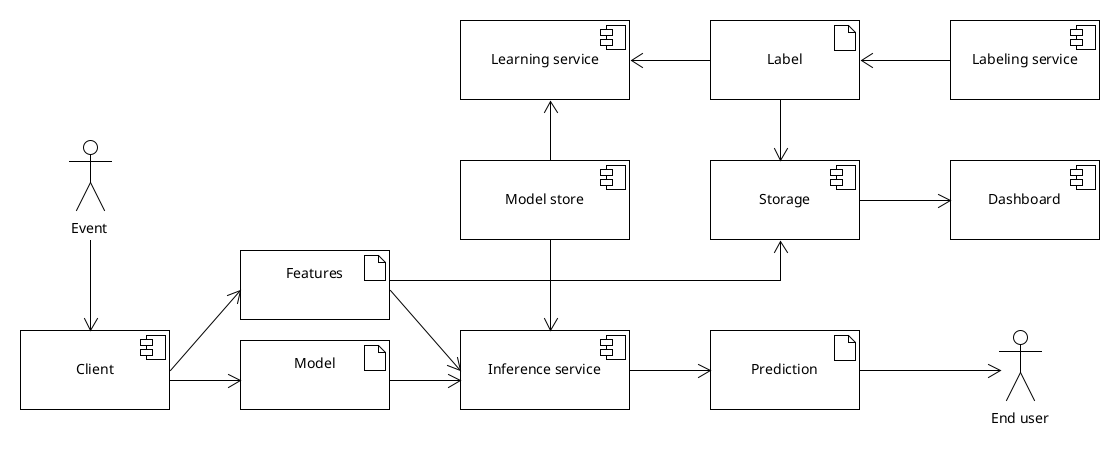
\includegraphics[width=\textwidth]{assets/analysis/incremental-learning.png}
    \caption{Incremental learning deployment architecture~\cite{gaia_online_2022}}
    \label{fig:online-learn-arch}
\end{figure}

Deployment of an online machine learning model alongside supporting services is different from established MLOps processes. Model store and Inference service components are supplemented with Labelling and Learning service~\cite{gaia_online_2022}. Their goal is to tune model parameters gradually as additional ground truth labels are provided. Labels can be provided later in a scheme called ``log and wait'', but data features are stored until such time.

\section{Datasets of machinery faults} \label{section:evaluation-datasets}
The experimentally designed features' relevancy is first proven in comparison to comprehensive benchmark datasets. There are a few standardized datasets used in the related work, e.g. \cite{ribeiro_rotating_2017}.

\emph{MaFaulDa} dataset combines vibration and acoustic measurements of the shaft in deviating positions and bearing abnormalities. \emph{CWRU dataset} focuses solely on faults in ball bearings. Another less known dataset concerns shaft unbalance, but compared to the previous two, it demonstrates behavior during speed up.

\subsection{Machinery Fault Database}
MaFaulDa~\cite{mafaulda_dataset} is a collection of 1951 multivariate time series for 4 different operational conditions on rotor kit Alignment Balance Vibration Trainer (ABVT)~(Fig.~\ref{fig:mafaulda-simulator}). Each series has 5~seconds in duration and is captured at 50 kHz. Vibration signals were obtained with piezoelectric accelerometers with a linear response up to 10~kHz, amplitude range to $\pm$490 $\mathrm{m/s}^2$, and resolution step of 10.2~mV per $\mathrm{m/s}^2$.

\begin{figure}[h]
\centering
\begin{subfigure}[b]{0.48\textwidth}
	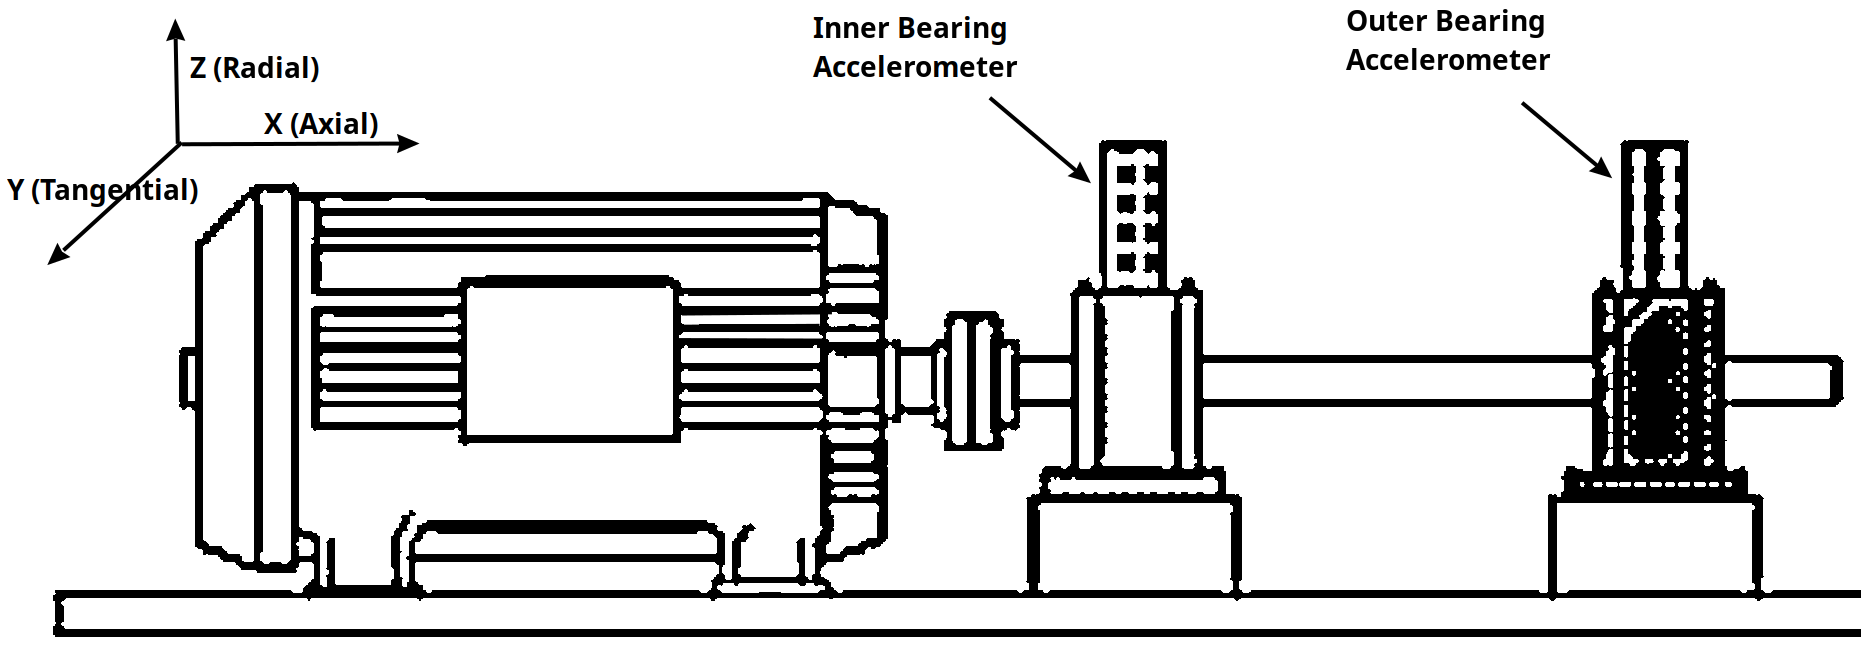
\includegraphics[width=\textwidth]{assets/analysis/mafaulda-simulator.png}
	\caption{Schematic diagram \cite{pestana-viana_influence_2016}}
\end{subfigure}
\hfill
\begin{subfigure}[b]{0.48\textwidth}
	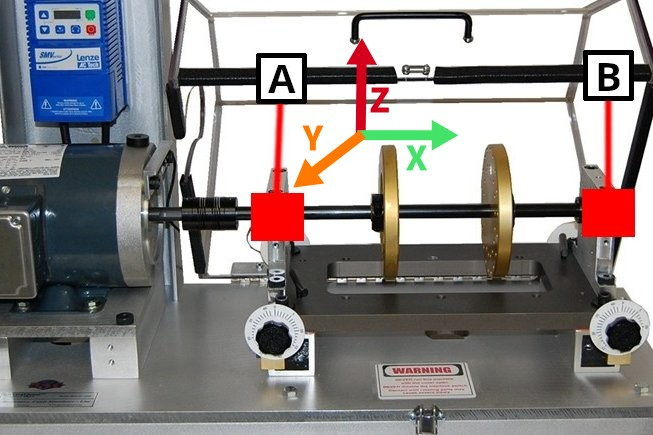
\includegraphics[width=\textwidth]{assets/design/sensor/mafaulda-simulator.jpg}
	\caption{Mechanical construction \cite{noauthor_spectraquest_nodate}}
\end{subfigure}
\caption{Machinery fault simulator for MaFaulDa}
\label{fig:mafaulda-simulator}
\end{figure}

Observations were conducted on three cardinal axes simultaneously with 2 sets of accelerometers, each one associated with one bearing (inner and outer bearings)~(Fig.~\ref{fig:mafaulda-simulator}). Additionally, a magnetic speedometer produced a pulse on shaft turn. The cardioid condenser microphone recorded sound emissions at a frequency range 20~Hz - 20~kHz. Sensors were fed into a four-channel dynamic signal acquisition module.

Columns in the dataset are organized as depicted in table~\ref{tab:mafaulda-columns}. Machine rotational speeds were kept constant during a particular measurement, but covered a range from 737 to 3686~rpm with steps of approximately 60 rpm (equiv. 10~Hz - 60~Hz)~\cite{pestana-viana_influence_2016}. The maximal rotational frequency achieved with a high unbalance load is 3300 rpm.

\begin{table}[h]
\renewcommand{\arraystretch}{1.2}
\centering
\begin{tabular}{|l|l|}
\hline
\textbf{Columns} & \textbf{Description}                                                                                                                                               \\ \hline
1.               & \begin{tabular}[c]{@{}l@{}}Pulse with modulation of speedometer signal \\ to estimate rotation frequency  (in TTL levels)\end{tabular}                              \\ \hline
2., 3., 4.       & \begin{tabular}[c]{@{}l@{}}Underhang bearing accelerometer \\ (inner - between the rotor and motor)\\ - axial, radial, tangential direction\end{tabular}           \\ \hline
5., 6., 7.       & \begin{tabular}[c]{@{}l@{}}Overhang bearing accelerometer \\ (outer - outside most position after the rotor)\\ - axial, radial, tangential direction\end{tabular} \\ \hline
8.               & Microphone                                                                                                                                                         \\ \hline
\end{tabular}
\caption{MaFaulDa description of columns}
\label{tab:mafaulda-columns}
\end{table}

This database contains normal operating conditions, faults out of unbalance, horizontal and vertical shaft misalignment, and three types of faulty bearings in inner and outer positions: outer track, inner track, rolling elements~\cite{pestana-viana_influence_2016}.

\begin{itemize}
\itemsep0pt

\item \textbf{Normal} conditions are baseline without the adverse effect of fault at 49 different rotation speeds.

\item \textbf{Unbalance} shaft time series uses 8 unbalancing weights from 6 to 35 grams and varying 45 - 49 speeds for each weight, adding to 333 mass unbalance loads.

\item \textbf{Vertical misalignment} set comprises 50 signals each (or 51 in one instance) obtained under displacements: 0.51, 0.63, 1.40, 1.90, 1.27, 1.78 mm.

\item \textbf{Horizontal misalignment} signals were recorded under displacements: 0.50, 1.00, 1.50, 2.00 mm, each with 49 different speeds (or 50 in one instance)~\cite{pestana-viana_influence_2016}.

\item \textbf{Bearing faults} are unnoticeable without unbalance. Therefore, weights of 6, 20, and 35 grams were attached to induce a detectable effect. Each mass was combined with cage, outer race, and ball faults at multiple rotation speeds, usually at 50 different speeds.
\end{itemize}


\subsection{CWRU bearings dataset}
In Case Western Reserve University (CWRU) bearing dataset~\cite{cwru_dataset} recordings were made of a fan end and drive end bearings under motor loads of 0, 1, 2, and 3~Horsepower (equivalently 0, 0.75, 1.49, 2.24~kW). Shaft speed was unaltered in all experiments, but it fluctuated between 1720 and 1797~rpm (approx. 29~Hz).

\begin{figure}[h]
\begin{subfigure}[b]{0.48\textwidth}
	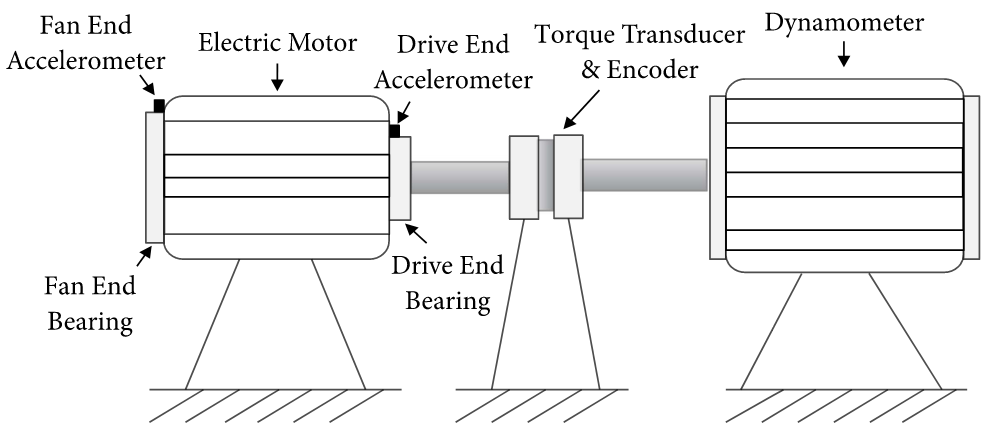
\includegraphics[width=\textwidth]{assets/analysis/cwru-test-stand-2.png}
	\caption{Schematic diagram \cite{song_bearing_2022}}
\end{subfigure}
\hfill
\begin{subfigure}[b]{0.48\textwidth}
	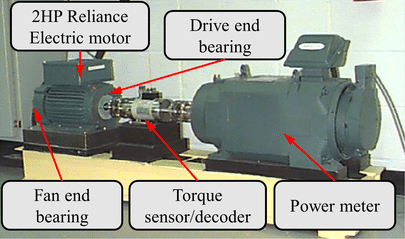
\includegraphics[width=\textwidth]{assets/analysis/cwru-test-stand.png}
	\caption{Mechanical construction \cite{yuhong_new_2021}}
\end{subfigure}
\caption{CWRU machine apparatus}
\label{fig:cwru-simulator}
\end{figure}

Single point defects were created with diameters of 0.007, 0.014, 0.021, 0.028, and 0.040 inches (equivalently 0.18, 0.36, 0.72, 1.02 mm). Fault locations on bearings are in the inner raceway, in the outer raceway directly and orthogonally relative to the load zone, and on rolling ball elements~(Fig.~\ref{fig:cwru-simulator})~\cite{jamil_feature-based_2021}.

\begin{table}[h]
\centering
\renewcommand{\arraystretch}{1.2}
\begin{tabular}{|l|l|}
\hline
\textbf{Columns} & \textbf{Description}                 \\ \hline
1. DE        & Drive end accelerometer samples 		\\ \hline
2. FE        & Fan end accelerometer samples   			\\ \hline
3. BA        & Base accelerometer samples (optional)   \\ \hline
4. RPM     & Rotation speed of the motor in rpm        \\ \hline
\end{tabular}
\caption{CWRU dataset description of columns}
\label{tab:cwru-columns}
\end{table}

The sampling frequency during baseline set, drive end, and fan end bearing capture is 12 kHz. For drive end bearings, samples were taken at 48 kHz. The duration of the time series varies from 5 to 40 seconds. Drive end and fan end bearing signals are measured in each experiment. Accelerometer was sometimes mounted on the supporting baseplate.

\subsection{Unbalance of the rotating shaft}
Unbalance Detection of a Rotating Shaft~\cite{unbalance_shaft} is a Kaggle dataset that simulates 4 different unbalance strengths.
\begin{figure}[h]
\centering
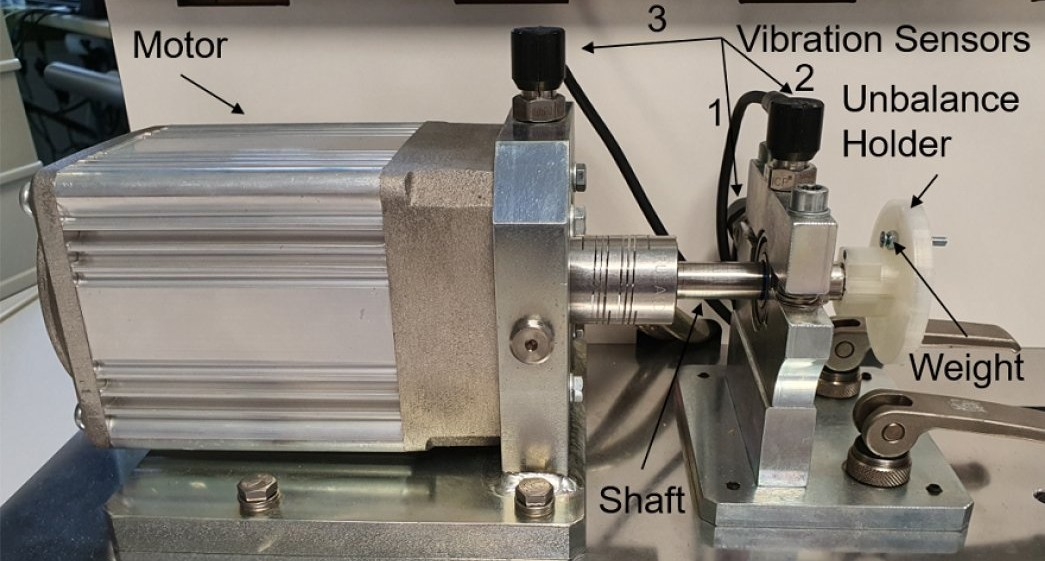
\includegraphics[width=0.7\textwidth]{assets/analysis/rotating-shaft.jpg}
\caption{Motor driving shaft in unbalance measurement \cite{mey_machine_2020}}
\label{fig:rotating-shaft}
\end{figure}

The setup is shown in Fig.~\ref{fig:rotating-shaft}. A mass of 3.28 grams (or 6.61 grams during the severe unbalance test) is attached to the unbalance holder in 5 sets (numbered 0 - 4) on the radii 0, 14, 18.5, 23, 23 mm. The rotation speed of the motor is perpetually rising between 630 and 2330 rpm in development datasets (marked with suffix D) and speeds from 1060 to 1900 rpm in the evaluation datasets (suffix E). The vibrations were recorded at a sampling rate of 4~kHz~\cite{mey_machine_2020}.

\begin{table}[h]
\centering
\renewcommand{\arraystretch}{1.2}
\begin{tabular}{|l|l|}
\hline
\textbf{Columns} & \textbf{Description}                      \\ \hline
1. V\_in         & Input voltage to the motor controller (V) \\ \hline
2. Measured\_RPM & Rotation speed of the motor (rpm)  \\ \hline
3. Vibration\_1  & 1. Vibration sensor (samples)             \\ \hline
4. Vibration\_2  & 2. Vibration sensor (samples)             \\ \hline
5. Vibration\_3  & 3. Vibration sensor (samples)             \\ \hline
\end{tabular}
\caption{``Unbalance on the rotating shaft'' dataset description of columns}
\end{table}

The accelerometers used are piezoelectric and have a frequency range of up to 10 kHz, dynamic range of $\pm$490 $m/s^2$, and resolution step of 10.2~mV per $\mathrm{m/s}^2$. These sensor parameters are the same as in the case of MaFaulDa. In total, three different uniaxial accelerometers are mounted on the motor housing.

